%Template para TCC CIC UFRGS
%Author: Lucas Schnorr (Adaptado para overleaf por Rubens dos Santos)

% exemplo genérico de uso da classe iiufrgs.cls
% $Id: iiufrgs.tex,v 1.1.1.1 2005/01/18 23:54:42 avila Exp $
%
% This is an example file and is hereby explicitly put in the
% public domain.
%
\documentclass[cic,tc]{iiufrgs}
% Para usar o modelo, deve-se informar o programa e o tipo de documento.
% Programas :
% * cic       -- Graduação em Ciência da Computação
% * ecp       -- Graduação em Ciência da Computação
% * ppgc      -- Programa de Pós Graduação em Computação
% * pgmigro   -- Programa de Pós Graduação em Microeletrônica
%
% Tipos de Documento:
% * tc                -- Trabalhos de Conclusão (apenas cic e ecp)
% * diss ou mestrado  -- Dissertações de Mestrado (ppgc e pgmicro)
% * tese ou doutorado -- Teses de Doutorado (ppgc e pgmicro)
% * ti                -- Trabalho Individual (ppgc e pgmicro)
%
% Outras Opções:
% * english    -- para textos em inglês
% * openright  -- Força início de capítulos em páginas ímpares (padrão da
% biblioteca)
% * oneside    -- Desliga frente-e-verso
% * nominatalocal -- Lê os dados da nominata do arquivo nominatalocal.def


% Use unicode
\usepackage[utf8]{inputenc}   % pacote para acentuação

% Necessário para incluir figuras
\usepackage{graphicx}         % pacote para importar figuras

\usepackage{times}            % pacote para usar fonte Adobe Times
% \usepackage{palatino}
% \usepackage{mathptmx}       % p/ usar fonte Adobe Times nas fórmulas

\usepackage[alf,abnt-emphasize=bf]{abntex2cite}	% pacote para usar citações abnt
\usepackage{amsmath}          % pacote para equações (cases, align, etc.)
\usepackage{amssymb}          % pacote para símbolos matemáticos (\mathbb, etc.)

%
% Informações gerais
%
\title{Estratégias de Gerenciamento de Tempo por Lance para Agentes MCTS no Jogo Gomoku}

\author{da Silveira}{Arthur Tonial}


\advisor[Prof.~Dr.]{Ribas}{Renato Perez}
% \coadvisor[Prof.~Dr.]{Sobrenome}{Nome}

\location{Porto Alegre}{RS}
\date{junho}{2026}

%
% palavras-chave
% iniciar todas com letras minúsculas, exceto no caso de abreviaturas
\keyword{Monte Carlo Tree Search}
\keyword{gerenciamento de tempo}
\keyword{Gomoku}
\keyword{jogos de tabuleiro}
\keyword{inteligência artificial}

%
% inicio do documento
%
\begin{document}

% folha de rosto
\maketitle

% dedicatoria
\clearpage
\begin{flushright}
    \mbox{}\vfill
    {\sffamily\itshape
      ``If I have seen farther than others,\\
      it is because I stood on the shoulders of giants.''\\}
    --- \textsc{Sir~Isaac Newton}
\end{flushright}

% agradecimentos
\chapter*{Agradecimentos}
Agradeço ao \LaTeX\ por não ter vírus de macro\ldots



% resumo na língua do documento
\begin{abstract}
O Monte Carlo Tree Search (MCTS) é um algoritmo \emph{anytime} para jogos: dado mais tempo por turno, tende a produzir decisões de maior qualidade. Em partidas competitivas com orçamento de tempo fixo por jogador, surge o problema de como distribuir esse orçamento entre os lances da partida. A estratégia mais comum — dividir o tempo restante igualmente — ignora que posições com ameaças táticas imediatas são muito mais críticas do que lances de abertura, onde o espaço de busca é vasto e as consequências são difusas.

Este trabalho propõe e compara quatro estratégias de alocação de tempo por lance aplicadas a um agente MCTS no Gomoku 15×15: (i) uniforme (\emph{flat}), utilizada como \emph{baseline}; (ii) proporcional, que escala a alocação com o preenchimento do tabuleiro; (iii) por fase, que aplica multiplicadores distintos na abertura, meio do jogo e final; e (iv) crítica, que detecta ameaças de 4-em-linha aberta e dobra o tempo alocado nesses lances. Cada estratégia foi avaliada em torneios de 400 partidas contra o \emph{baseline} uniforme em três orçamentos de tempo — 30, 60 e 120 segundos por jogador — com alternância de cores para controlar o viés do primeiro movimento, totalizando 3600 partidas. Os resultados a seguir referem-se ao experimento principal (60 segundos).

A estratégia crítica obteve 61,8\% de vitórias ($p < 0{,}001$), superando o \emph{baseline} de forma consistente em ambas as cores. A estratégia por fase obteve 40,2\% ($p < 0{,}001$), sendo significativamente inferior ao \emph{baseline}: o excesso de tempo investido no meio do jogo esgota o orçamento antes dos lances decisivos do final. A estratégia proporcional obteve 52,2\% ($p = 0{,}37$), resultado estatisticamente indistinguível do \emph{baseline}.

O achado central é que a qualidade do sinal de alocação importa mais do que o volume de tempo redistribuído. A estratégia crítica, com um sinal binário simples ativado em apenas 20\% dos lances, superou estratégias que redistribuem tempo de forma mais contínua ao longo da partida. A hipótese do trabalho é confirmada parcialmente: alocação inteligente supera o \emph{baseline} quando o sinal utilizado é específico e preciso o suficiente.
\end{abstract}

% resumo na outra língua
\begin{englishabstract}{Time Management Strategies per Move for MCTS Agents in Gomoku}{Monte Carlo Tree Search. time management. Gomoku. board games. artificial intelligence}
Monte Carlo Tree Search (MCTS) is an anytime algorithm for games: given more time per turn, it tends to produce higher-quality decisions. In competitive settings with a fixed time budget per player, the problem of how to distribute this budget across the moves of a game arises. The most common strategy — dividing the remaining time equally among estimated remaining moves — ignores that positions with immediate tactical threats are far more critical than opening moves, where the search space is vast and consequences are diffuse.

This work proposes and compares four per-move time allocation strategies applied to an MCTS agent in 15×15 Gomoku: (i) uniform (flat), used as baseline; (ii) proportional, scaling allocation with board fill ratio; (iii) phase-based, applying distinct multipliers for the opening, midgame, and endgame; and (iv) critical, detecting open four-in-a-row threats and doubling the time allocated to those moves. Each strategy was evaluated in tournaments of 400 games against the flat baseline across three time budgets — 30, 60, and 120 seconds per player — with color alternation to control the first-move advantage, totalling 3600 games. Results below refer to the main experiment (60 seconds).

The critical strategy achieved 61.8\% wins ($p < 0.001$), consistently outperforming the baseline in both colors. The phase strategy achieved 40.2\% wins ($p < 0.001$), performing significantly worse than the baseline: overspending in the midgame depletes the budget before the decisive endgame moves. The proportional strategy achieved 52.2\% wins ($p = 0.37$), statistically indistinguishable from the baseline.

The central finding is that the quality of the allocation signal matters more than the volume of time redistributed. The critical strategy, using a simple binary signal activated on only 20\% of moves, outperformed strategies that redistribute time continuously throughout the game. The work's hypothesis is partially confirmed: intelligent allocation outperforms the baseline when the signal is specific and precise enough.
\end{englishabstract}

% lista de figuras
\listoffigures

% lista de tabelas
\listoftables

% lista de abreviaturas e siglas
\begin{listofabbrv}{MCTS}
    \item[IA]   Inteligência Artificial
    \item[MCTS] Monte Carlo Tree Search
    \item[UCB]  Upper Confidence Bound
    \item[UCB1] Upper Confidence Bound 1
    \item[UCT]  Upper Confidence Bound for Trees
    \item[GGP]  General Game Playing
\end{listofabbrv}

% idem para a lista de símbolos
% \begin{listofsymbols}{$\alpha\beta\pi\omega$}
%     \item[$\sum{\frac{a}{b}}$] Somatório do produtório
%     \item[$\alpha\beta\pi\omega$] Fator de inconstância do resultado
% \end{listofsymbols}

% sumario
\tableofcontents

% -----------------------------------------------------------------------
% CAPÍTULO 1 — Introdução
% -----------------------------------------------------------------------
\chapter{Introdução}

A Inteligência Artificial (IA) tem avançado de forma expressiva nas últimas décadas, permeando domínios que vão da medicina ao planejamento logístico. Um dos ambientes que mais contribuiu para o desenvolvimento dessa área são os jogos: sua estrutura formal e adversarial oferece um laboratório controlado no qual algoritmos podem ser avaliados de forma rigorosa e comparável. Este trabalho insere-se nessa tradição, investigando um aspecto específico e pouco explorado de agentes automáticos para jogos: a distribuição inteligente do orçamento de tempo entre os movimentos de uma partida.

% ---
\section{Inteligência Artificial em Jogos}
\label{sec:intro_games}

Jogos de tabuleiro constituem um \textit{benchmark} clássico para agentes de IA desde as primeiras décadas da área. \citet{shannon1950programming} foi pioneiro ao analisar formalmente o problema de jogar xadrez por computador, estabelecendo os fundamentos teóricos que viriam a embasar décadas de pesquisa. A representação de uma partida como uma árvore de estados — com alternância de movimentos entre dois adversários — é a estrutura central de toda essa linha de trabalho.

O algoritmo Minimax e suas extensões (Seção~\ref{sec:minimax}) formalizaram essa estrutura e, combinados com funções de avaliação heurísticas cuidadosamente elaboradas, permitiram que programas de Xadrez atingissem nível de grande mestre (GM). Com o surgimento da Busca em Árvore de Monte Carlo (\textit{Monte Carlo Tree Search} --- MCTS) \cite{coulom2006efficient,kocsis2006bandit}, porém, abriu-se uma nova fronteira: ao estimar o valor de posições por simulação estatística em vez de busca exaustiva, o MCTS dispensou a necessidade de funções de avaliação explícitas e demonstrou saltos de desempenho expressivos em jogos de alta complexidade, como o Go \cite{gelly2006modification}. Esse avanço culminou em marcos históricos como o AlphaGo e o AlphaZero, que combinaram MCTS com aprendizado profundo para superar os melhores jogadores humanos em Go e Xadrez.

Este trabalho foca exclusivamente em agentes baseados em MCTS sem aprendizado de máquina. O objetivo é estudar o comportamento do algoritmo em condições de tempo limitado — um problema que permanece relevante e aberto independentemente das capacidades de redes neurais.

% ---
\section{Motivação e Justificativa}
\label{sec:motivation}

O MCTS foi amplamente estudado sob diferentes ângulos: a formulação do critério de seleção UCT (\emph{Upper Confidence Bound for Trees}) \cite{kocsis2006bandit}, variantes de expansão e simulação(\emph{rollout}), e aplicações a domínios além dos jogos \cite{browne2012survey}. Uma dimensão prática, porém, recebeu atenção comparativamente limitada: o gerenciamento de tempo por lance.

Em partidas competitivas, o orçamento de tempo total por jogador é fixo e deve ser distribuído entre todos os lances da partida. Como o MCTS é um algoritmo \emph{anytime} — pode ser interrompido a qualquer momento e retorna o melhor movimento encontrado até então — o tempo disponível por turno é o recurso natural de controle: mais tempo implica mais iterações e, em geral, estimativas mais precisas e decisões de maior qualidade. A questão que se coloca é como distribuir esse orçamento de forma eficaz ao longo de uma partida.

A estratégia mais simples — dividir o tempo restante igualmente entre os movimentos estimados — é também a mais comum na prática \cite{browne2012survey}. Ela ignora, porém, que nem todos os lances têm a mesma importância: posições com ameaças táticas imediatas são fatais se mal respondidas, enquanto lances de abertura com tabuleiro esparso tendem a ter consequências mais difusas. Investir tempo adicional nos momentos críticos e economizar nos demais poderia, em teoria, aumentar a qualidade agregada das decisões sem alterar o orçamento total. Essa lacuna motiva o presente trabalho.

A hipótese central é que estratégias de alocação sensíveis ao estado do jogo — em particular, aquelas capazes de identificar momentos táticos críticos — superam a alocação uniforme em taxa de vitórias. A motivação é direta: se o valor marginal de uma iteração adicional do MCTS é maior em posições de alta importância tática, redistribuir tempo para esses momentos deve aumentar a qualidade agregada das decisões sem alterar o orçamento total.

% ---
\section{Objetivos}
\label{sec:objectives}

\textbf{Objetivo geral}: Comparar estratégias de alocação de tempo por lance em agentes MCTS aplicados ao Gomoku e quantificar o impacto de cada abordagem na taxa de vitórias.

\textbf{Objetivos específicos}:

\begin{itemize}
    \item Implementar quatro variantes de alocação de tempo (uniforme, proporcional, por fase e crítica) sobre um agente MCTS comum;
    \item Desenvolver uma infraestrutura de torneio controlada para coleta sistemática de dados;
    \item Medir o impacto de cada estratégia em duelos com condições controladas — orçamento fixo, alternância de cores e número de partidas suficiente para inferência estatística;
    \item Analisar os \emph{trade-offs} e limitações de cada abordagem à luz dos resultados obtidos.
\end{itemize}

% ---
\section{Organização do Trabalho}
\label{sec:organization}

O restante deste trabalho está organizado da seguinte forma. O Capítulo~\ref{chap:background} apresenta os conceitos fundamentais: busca em árvores de jogo, o algoritmo MCTS, estratégias de gerenciamento de tempo identificadas na literatura e as propriedades do jogo Gomoku. O Capítulo~\ref{chap:proposal} formaliza o problema de alocação de tempo, descreve a arquitetura conceitual da solução e apresenta as quatro estratégias propostas. O Capítulo~\ref{chap:implementation} detalha a implementação do sistema. O Capítulo~\ref{chap:results} apresenta os resultados experimentais e sua análise. Por fim, o Capítulo~6 sintetiza as conclusões do trabalho e aponta direções para pesquisa futura.

% -----------------------------------------------------------------------
% CAPÍTULO 2 — Fundamentação Teórica
% -----------------------------------------------------------------------
\chapter{Fundamentação Teórica}
\label{chap:background}

Este capítulo apresenta os conceitos necessários para a compreensão do trabalho. A Seção~\ref{sec:minimax} introduz o problema de busca em árvores de jogo e o algoritmo Minimax como abordagem clássica, estabelecendo a base conceitual sobre a qual o MCTS se apoia. A Seção~\ref{sec:mcts} descreve o Monte Carlo Tree Search, algoritmo central deste trabalho. A Seção~\ref{sec:timemanagement} discute o problema de gerenciamento de tempo em jogos e as estratégias de alocação propostas na literatura. Por fim, a Seção~\ref{sec:gomoku} apresenta o jogo Gomoku e suas propriedades relevantes para o contexto deste trabalho.

% ---
\section{Busca em Árvores de Jogo}
\label{sec:minimax}

A busca em árvores de jogo é o paradigma central dos agentes automáticos para jogos de dois jogadores com informação perfeita --- aqueles em que o estado completo do jogo é visível a ambos os jogadores a qualquer momento, sem elementos ocultos ou aleatoriedade, como ocorre no Xadrez, no Go e no Gomoku. Esta seção apresenta o problema na sua formulação clássica — o algoritmo Minimax e sua principal otimização, a poda alfa-beta — que constituem a fundação histórica da área e o ponto de partida conceitual para compreender as motivações do MCTS. A limitação fundamental dessas abordagens em domínios de alta complexidade, discutida na Seção~\ref{sec:minimax_limits}, é precisamente o que motivou o desenvolvimento do MCTS como alternativa baseada em simulação.

Jogos de dois jogadores com informação perfeita e soma zero constituem um dos domínios mais estudados em Inteligência Artificial. Nesse modelo, dois agentes se alternam realizando movimentos em um estado compartilhado; o ganho de um implica a perda equivalente do outro. Xadrez, damas, Go e Gomoku são exemplos canônicos. A representação natural de uma partida é uma árvore de jogo: cada nó corresponde a um estado e cada aresta a um movimento legal, com folhas representando estados terminais cujo valor é determinado pelo resultado da partida.

O algoritmo Minimax \cite{russell2016artificial} percorre essa árvore recursivamente, atribuindo a cada nó o melhor resultado possível sob jogo ótimo de ambos os lados (Figura~\ref{fig:minimax_tree}). O jogador maximizador (\emph{MAX}) escolhe o movimento de maior valor; o minimizador (\emph{MIN}), o de menor (Equação~\ref{eq:minimax}):

\begin{equation}
    \label{eq:minimax}
    V(n) =
    \begin{cases}
        \text{utilidade}(n)             & \text{se } n \text{ é folha}      \\
        \max_{s \in \text{filhos}(n)} V(s) & \text{se é turno de MAX}       \\
        \min_{s \in \text{filhos}(n)} V(s) & \text{se é turno de MIN}
    \end{cases}
\end{equation}

\begin{figure}[htbp]
    \centering
    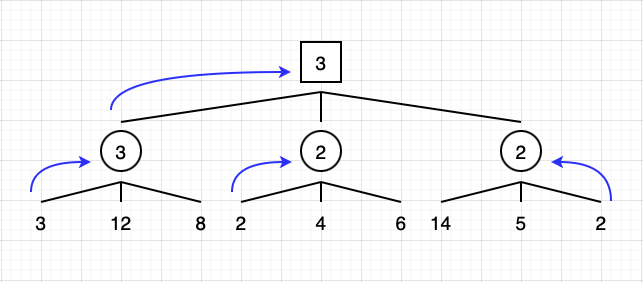
\includegraphics[width=0.8\textwidth]{images/minimax}
    \caption{Exemplo de árvore Minimax com dois níveis de profundidade. Nós quadrados representam o jogador MAX; nós circulares, o jogador MIN. Os valores das folhas são propagados de baixo para cima.}
    \label{fig:minimax_tree}
        \legend{Fonte: Elaborado pelo autor}
\end{figure}

Para jogos finitos, o Minimax é teoricamente ótimo, mas a busca exaustiva é inviável para fator de ramificação elevado — o Xadrez, por exemplo, possui fator médio de 35 e duração de 80 lances, produzindo $35^{80}$ folhas \cite{shannon1950programming}. Na prática, a busca é limitada a uma profundidade predefinida e os nós não terminais são avaliados por uma função heurística $h(n)$. A principal otimização é a poda alfa-beta \cite{knuth1975analysis}, que mantém dois limitantes $\alpha$ (melhor para MAX) e $\beta$ (melhor para MIN) e descarta ramos que não podem influenciar a decisão da raiz. No melhor caso, reduz a complexidade de $O(b^d)$ para $O(b^{d/2})$, efetivamente dobrando a profundidade alcançável (Figura~\ref{fig:alpha_beta}).

\begin{figure}[htbp]
    \centering
    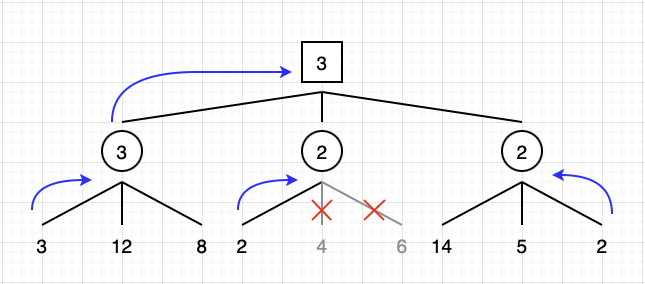
\includegraphics[width=0.8\textwidth]{images/alfabeta_pruning.png}
    \caption{Ilustração da poda alfa-beta sobre uma árvore Minimax. Os ramos marcados em cinza são podados por não poderem influenciar a decisão da raiz, dado os limites $\alpha$ e $\beta$ já estabelecidos.}
    \label{fig:alpha_beta}
    \legend{Fonte: Elaborado pelo autor}
\end{figure}

\subsection{Limitações do Minimax em jogos complexos}
\label{sec:minimax_limits}

Apesar de sua eficácia no Xadrez, o Minimax com poda alfa-beta apresenta limitações fundamentais que o tornam inadequado para jogos como Go e Gomoku. Primeiro, o fator de ramificação do Go em um tabuleiro $19 \times 19$ chega a 361 no primeiro movimento, tornando a busca profunda computacionalmente proibitiva mesmo com poda. Segundo, e mais criticamente, a definição de uma função de avaliação heurística de qualidade para esses jogos é extremamente difícil: no Go, por exemplo, não existe uma heurística largamente aceita que capture com fidelidade a qualidade de uma posição.

Esses obstáculos motivaram o desenvolvimento de abordagens baseadas em simulação, que dispensam a necessidade de uma função de avaliação explícita ao estimar o valor de um estado através de partidas aleatórias \cite{browne2012survey}.

% ---
\section{Monte Carlo Tree Search}
\label{sec:mcts}

O MCTS é uma família de algoritmos de busca que combina a expansão seletiva de uma árvore de jogo com a estimativa de valores por simulação estocástica \cite{browne2012survey}. Diferentemente do Minimax, o MCTS não requer função de avaliação: o valor de um estado é estimado pela proporção de vitórias obtidas em simulações (chamadas \emph{rollouts}) iniciadas a partir daquele estado.

O MCTS foi proposto de forma seminal por \citet{coulom2006efficient}, que introduziu o uso de simulações Monte Carlo combinadas com busca em árvore para jogos de tabuleiro. A variante Limite de Confiança Superior para Árvores (\emph{Upper Confidence Bound for Trees} --- UCT), que se tornou a formulação dominante, foi proposta por \citet{kocsis2006bandit} ao aplicar o critério Limite de Confiança Superior 1 (\emph{Upper Confidence Bound 1} --- UCB1) à seleção de nós na árvore. A aplicação ao Go por \citet{gelly2006modification} demonstrou saltos substanciais de desempenho em relação às abordagens anteriores, e o algoritmo passou a ser adotado em uma ampla variedade de domínios \cite{browne2012survey}.

\subsection{Visão geral do MCTS}
\label{sec:mcts_overview}

O MCTS opera iterativamente, construindo uma árvore de busca parcial a partir do estado raiz. Cada iteração compreende quatro fases:

\begin{enumerate}
    \item \textbf{Seleção}: a partir da raiz, o algoritmo desce a árvore selecionando em cada nó o filho que maximiza um critério de seleção — tipicamente UCB1 (detalhado na Seção~\ref{sec:ucb1}) — até alcançar um nó folha ou um nó não totalmente expandido.

    \item \textbf{Expansão}: se o nó selecionado não é terminal, um ou mais filhos são adicionados à árvore, representando movimentos legais ainda não explorados.

    \item \textbf{Simulação} (\emph{rollout}): a partir do nó expandido, uma partida é simulada até o estado terminal, geralmente com uma política de movimentos aleatória ou levemente guiada por heurísticas.

    \item \textbf{Retropropagação}: o resultado da simulação é propagado de volta ao longo do caminho percorrido, atualizando os contadores de visitas $N(v)$ e de valor acumulado $W(v)$ de cada nó.
\end{enumerate}

Ao final de um orçamento de iterações ou tempo, o algoritmo retorna o movimento correspondente ao filho da raiz mais visitado, que tende a ser o de maior valor estimado (Figura~\ref{fig:mcts_cycle}).

\begin{figure}[htbp]
    \centering
    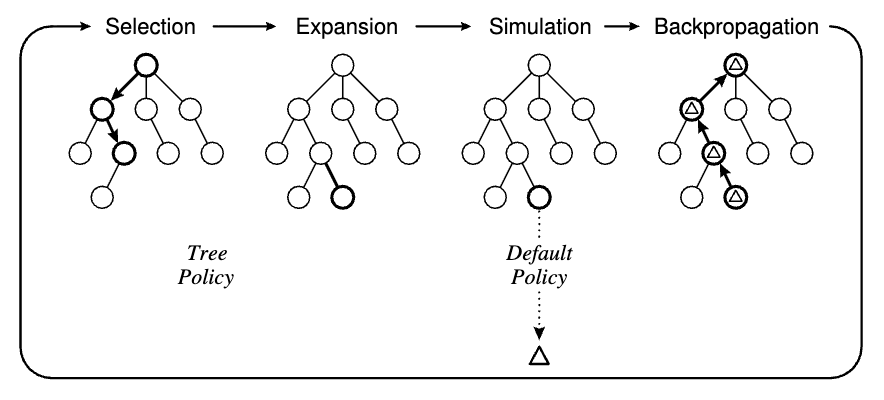
\includegraphics[width=0.75\textwidth]{images/MCTS_iteration.png}
    \caption{Ciclo de uma iteração do MCTS composto pelas quatro fases: seleção, expansão, simulação (\emph{rollout}) e retropropagação.}
    \label{fig:mcts_cycle}
    \legend{Fonte: Extraído de \citeauthor{browne2012survey} (\citeyear{browne2012survey})}
\end{figure}

\subsection{UCB1 e o dilema exploração-explotação}
\label{sec:ucb1}

O critério de seleção é o coração do MCTS. O problema pode ser formulado como um \emph{multi-armed bandit}: cada filho de um nó é um braço cujo valor real é desconhecido e deve ser estimado por tentativas sucessivas. O UCB1, proposto por \citet{auer2002finite}, balanceia a exploração de nós promissores com a exploração de nós pouco visitados (Equação~\ref{eq:ucb1}):

\begin{equation}
    \text{UCB1}(v) = \frac{W(v)}{N(v)} + C \cdot \sqrt{\frac{\ln N(\text{pai}(v))}{N(v)}}
\label{eq:ucb1}
\end{equation}

onde $W(v)/N(v)$ é a taxa de vitórias estimada do nó $v$ (\emph{explotação}), e o segundo termo favorece nós pouco visitados em relação aos seus irmãos (\emph{exploração}). A constante $C$ controla o balanço entre os dois termos; o valor $C = \sqrt{2}$ é teoricamente motivado \cite{kocsis2006bandit} e amplamente utilizado na prática.

A adaptação do UCB1 para árvores de jogo, denominada UCT, consiste em aplicar a Equação~\ref{eq:ucb1} recursivamente em cada nó durante a fase de seleção, com a ressalva de que os valores são invertidos entre nós de perspectivas opostas, dado que vitória para um jogador é derrota para o outro. A Figura~\ref{fig:ucb1_curve} ilustra como o valor UCB1 varia em função do número de visitas para diferentes taxas de vitória estimadas; a Figura~\ref{fig:ucb1_bonus} mostra o comportamento isolado do termo de exploração.

\begin{figure}[htbp]
    \centering
    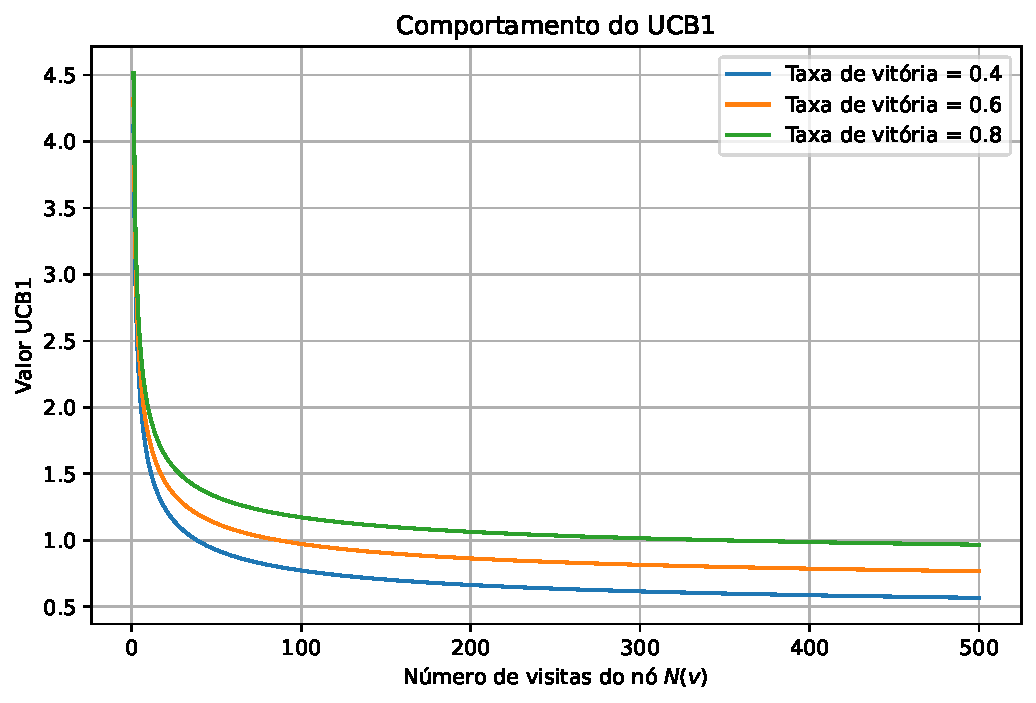
\includegraphics[width=0.8\textwidth]{images/ucb1_complete.pdf}
    \caption{
        Valor do UCB1 em função do número de visitas do nó $N(v)$ para diferentes taxas de vitória estimadas. O termo de exploração domina quando o nó foi pouco visitado e decai progressivamente à medida que mais simulações são realizadas.
    }
    \label{fig:ucb1_curve}
    \legend{Fonte: Elaborado pelo autor}
\end{figure}
\begin{figure}[htbp]
    \centering
    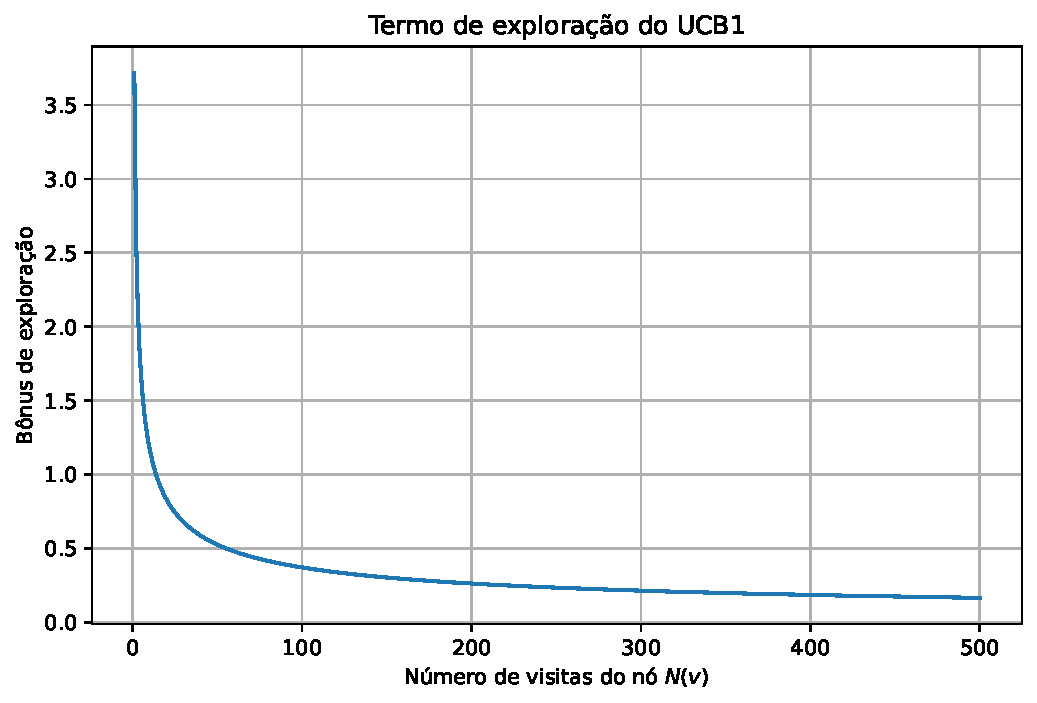
\includegraphics[width=0.8\textwidth]{images/ucb1_exploration_bonus.pdf}
    \caption{
        Termo de exploração do UCB1 em função do número de visitas do nó. O bônus de exploração é elevado para nós pouco visitados e diminui conforme o número de simulações aumenta.
    }
    \label{fig:ucb1_bonus}
    \legend{Fonte: Elaborado pelo autor}
\end{figure}

\subsection{MCTS como algoritmo \emph{anytime}}
\label{sec:mcts_anytime}

Uma propriedade fundamental do MCTS é sua natureza \emph{anytime}: o algoritmo pode ser interrompido a qualquer momento e retorna uma resposta válida — o movimento mais visitado até então. Em geral, a qualidade da resposta tende a melhorar com o número de iterações: mais simulações produzem estimativas de valor mais precisas e maior profundidade efetiva de busca. Essa relação não é, porém, garantida em toda configuração — ela depende da política de \emph{rollout}, da constante de exploração e da estrutura do espaço de busca.

Essa propriedade contrasta diretamente com o Minimax com profundidade fixa, que somente fornece resultado ao completar a busca até a profundidade estipulada. No MCTS, o recurso natural de controle é o tempo disponível: dado um orçamento de $T$ segundos por turno, o algoritmo executa o maior número possível de iterações dentro desse limite. Como a taxa de melhoria decresce com o número de iterações (retornos marginais decrescentes), a questão de como distribuir o orçamento total de tempo entre os movimentos de uma partida torna-se relevante — e é precisamente o problema abordado neste trabalho.

% ---
\section{Gerenciamento de Tempo em Jogos}
\label{sec:timemanagement}

O gerenciamento de tempo é o problema de decidir, a cada turno, quanto do orçamento disponível investir na busca pelo melhor movimento. Para agentes automáticos baseados em MCTS, essa decisão é especialmente relevante: como o algoritmo é \emph{anytime}, a qualidade da resposta tende a crescer com o tempo, mas o orçamento total por partida é finito e deve ser distribuído entre todos os lances. Esta seção apresenta o contexto histórico do controle de tempo em competições, os tipos de estratégias de alocação identificados na literatura e o estado da arte para agentes MCTS.

\subsection{Controle de tempo em competições}
\label{sec:timecontrol_history}

O controle de tempo é parte integrante das competições de jogos desde o século XIX. No Xadrez, o relógio foi introduzido em 1861 para evitar que partidas se prolongassem indefinidamente \cite{shannon1950programming}. Ao longo do tempo, diferentes modalidades de controle foram adotadas: tempo fixo por partida, tempo fixo por lance, e o sistema Fischer, no qual cada jogador recebe um bônus de tempo a cada lance realizado.

Essas modalidades impõem ao jogador — humano ou computador — o problema de alocação de tempo: dado um orçamento total finito $T$, quanto tempo dedicar a cada movimento? Jogadores humanos experientes intuitivamente gastam mais tempo em posições críticas e menos em lances óbvios. A formalização dessa estratégia para agentes automáticos é o objeto de estudo desta seção.

\subsection{Tipos de estratégias de alocação de tempo}
\label{sec:timealloc_types}

As estratégias de alocação de tempo para agentes de jogo podem ser organizadas em um espectro de crescente sofisticação. As principais categorias adotadas neste trabalho são descritas a seguir.

\textbf{Uniforme} (\emph{flat}): o tempo disponível é dividido igualmente entre os movimentos estimados restantes. Formalmente, se $T_r$ é o tempo restante e $\hat{N}$ é a estimativa de movimentos restantes para aquele jogador, o tempo alocado ao lance corrente é $t = T_r / \hat{N}$. Essa abordagem é simples, previsível e serve como \emph{baseline} natural para comparações.

\textbf{Proporcional}: variante do uniforme que se corrige ao longo da partida. Em vez de usar uma estimativa fixa de movimentos restantes, recalcula $\hat{N}$ com base na posição atual do tabuleiro, ajustando a alocação conforme a partida evolui.

\textbf{Baseada em fase}: aplica multiplicadores distintos sobre a alocação uniforme de acordo com a fase do jogo (abertura, meio, fim). A motivação é que o meio do jogo concentra as decisões táticas mais consequentes, merecendo maior investimento de tempo.

\textbf{Reativa} (ou baseada em criticidade): detecta posições táticas especiais — ameaças imediatas de vitória ou derrota — e aloca tempo extra nessas situações. Requer um critério de detecção de criticidade, que pode ir desde padrões simples (como sequências de $k-1$ peças em linha) até avaliações mais elaboradas.

\textbf{Adaptativa/aprendida}: aprende a distribuição ótima de tempo a partir de dados de partidas anteriores, tipicamente por aprendizado por reforço ou análise estatística. Essa abordagem está fora do escopo do presente trabalho, mas é apontada como direção futura relevante.

\subsection{Gerenciamento de tempo para MCTS}
\label{sec:timemanagement_mcts}

Apesar de sua importância prática, o problema de gerenciamento de tempo para agentes MCTS recebeu atenção relativamente limitada na literatura em comparação com outros aspectos do algoritmo. \citet{huang2010time} investigaram estratégias de alocação para um agente de Go baseado em MCTS, demonstrando que alocações adaptativas — que destinam mais tempo a posições com alta incerteza na estimativa de valor — superam a alocação uniforme em taxa de vitórias. \citet{finnsson2008simulation} abordaram o problema no contexto de Jogo Geral (\emph{General Game Playing} --- GGP), onde o agente deve jogar jogos desconhecidos em tempo limitado, e propuseram heurísticas baseadas na distribuição de visitas da árvore de busca para identificar lances que merecem atenção adicional.

\citet{browne2012survey} identificam o gerenciamento de tempo como um dos fatores práticos mais relevantes para o desempenho de agentes MCTS em competições, destacando que a maioria das implementações utiliza estratégias simples e que há espaço considerável para ganhos através de abordagens mais sofisticadas.

O presente trabalho instancia e compara experimentalmente quatro estratégias de alocação — uniforme, proporcional, por fase e crítica — sobre um agente MCTS aplicado ao Gomoku, com o objetivo de quantificar o impacto de cada abordagem na taxa de vitórias.

% ---
\section{O Jogo Gomoku}
\label{sec:gomoku}

\subsection{Regras e estrutura}
\label{sec:gomoku_rules}

Gomoku é um jogo de tabuleiro de dois jogadores jogado em um tabuleiro de $15 \times 15$ interseções. Os jogadores se alternam colocando peças de suas respectivas cores (preto e branco) em interseções vazias. Vence o jogador que formar primeiro uma sequência ininterrupta de cinco peças em linha — horizontal, vertical ou diagonal. A partida termina em derrota para um dos lados; empates são extremamente raros na prática.

Por convenção e em consonância com a vantagem do primeiro movimento, o jogador de peças pretas realiza o primeiro lance. \citet{allis1994searching} provou formalmente que, com jogo ótimo, o primeiro jogador vence em Gomoku sem restrições — empates são, portanto, praticamente inexistentes em jogo normal, o que é refletido nos resultados experimentais deste trabalho.

\subsection{Características relevantes para o MCTS}
\label{sec:gomoku_mcts}

O Gomoku apresenta propriedades que o tornam um domínio adequado para o estudo de estratégias de gerenciamento de tempo aplicadas ao MCTS.

\textbf{Fator de ramificação variável}: no início da partida, o número de movimentos legais é igual ao número de interseções vazias — até 225 no primeiro lance. Esse número decresce linearmente ao longo da partida, tornando a busca progressivamente mais profunda e precisa com o mesmo orçamento de tempo. Isso implica que a alocação de tempo no início da partida é proporcionalmente menos eficiente do que no final, o que motiva estratégias que considerem a fase do jogo.

\textbf{Fases distintas}: a partida pode ser dividida em fases com características estratégicas distintas. Na abertura, o tabuleiro é esparso e as decisões têm caráter posicional de longo prazo. No meio do jogo, surgem ameaças táticas diretas — sequências de três e quatro peças em linha — que demandam resposta imediata. No final, o tabuleiro está mais preenchido e as sequências críticas são mais frequentes. Essa estrutura justifica estratégias baseadas em fase.

\textbf{Padrões táticos críticos}: a ameaça de 4-em-linha aberta (quatro peças consecutivas com ambas as extremidades livres) constitui uma ameaça imediata de vitória que, se não bloqueada, resulta inevitavelmente em derrota. Da mesma forma, um jogador que cria duas ameaças simultâneas de 3-em-linha (denominado \emph{duplo três}) garante a vitória independentemente da resposta do oponente. Esses padrões motivam estratégias de alocação reativas que identificam posições críticas e destinam tempo adicional a elas (Figura~\ref{fig:gomoku_patterns}).

\begin{figure}[htbp]
    \centering
    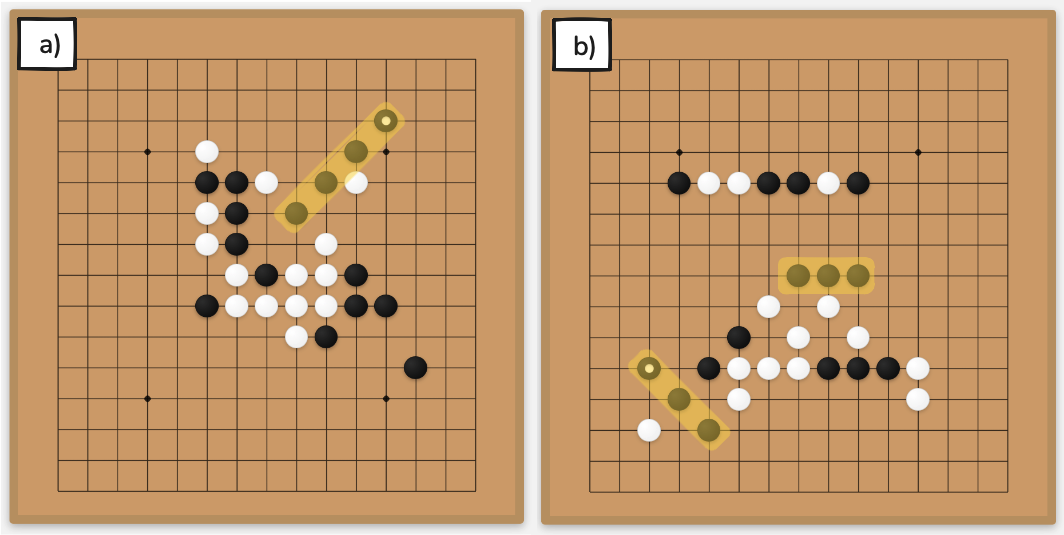
\includegraphics[width=0.8\textwidth]{images/Gomoku_boards.png}
    \caption{Exemplos de padrões táticos críticos no Gomoku em um tabuleiro $15 \times 15$: (a) sequência de quatro peças com extremidade aberta (\emph{4 aberto}), ameaça direta de vitória; (b) configuração de duplo-três, garantindo vitória independente da resposta do oponente.}
    \label{fig:gomoku_patterns}
    \legend{Fonte: Elaborado pelo autor}
\end{figure}

% -----------------------------------------------------------------------
% CAPÍTULO 3 — Proposta
% -----------------------------------------------------------------------
\chapter{Proposta}
\label{chap:proposal}

Este capítulo apresenta a proposta do trabalho. A Seção~\ref{sec:problem} formaliza o problema de alocação de tempo por lance no contexto de agentes MCTS. A Seção~\ref{sec:architecture} descreve a arquitetura conceitual da solução, com ênfase na separação entre política de tempo e motor de busca. A Seção~\ref{sec:strategies} apresenta e justifica as quatro estratégias de alocação propostas a partir das propriedades do domínio descritas no Capítulo~\ref{chap:background}.

% ---
\section{Definição Formal do Problema}
\label{sec:problem}

\subsection{Qualidade de decisão e tempo no MCTS}
\label{sec:quality_time}

O ponto de partida é a propriedade \emph{anytime} do MCTS (Seção~\ref{sec:mcts_anytime}): dado um prazo $t_i$ segundos para o lance $i$, o agente executa o maior número possível de iterações dentro desse limite e retorna o movimento mais visitado. Assume-se que a qualidade da decisão é uma função crescente do tempo disponível — mais iterações produzem estimativas de valor mais precisas e maior profundidade efetiva de busca. Adicionalmente, modela-se essa função como côncava: os ganhos de precisão tendem a ser decrescentes, pois as primeiras iterações amostreiam regiões do espaço de busca ainda completamente desconhecidas, enquanto iterações adicionais refinam estimativas já razoáveis, contribuindo cada vez menos para a qualidade da decisão final. Embora a concavidade de $Q(t)$ seja uma simplificação — a relação real depende da estrutura do espaço de busca, da política de \emph{rollout} e da constante de exploração —, ela é consistente com resultados empíricos na literatura \cite{browne2012survey} e serve como motivação teórica para o problema de alocação.

Essa característica tem uma consequência direta para o problema de alocação: redistribuir tempo de posições de baixo retorno marginal para posições de alto retorno marginal pode aumentar a qualidade agregada das decisões sem alterar o orçamento total. Formalmente, se $Q(t)$ denota a qualidade esperada de uma decisão com $t$ segundos de busca, e se assumirmos que $Q$ é côncava (retornos decrescentes), então para dois lances $i$ e $j$ com importâncias distintas $v_i > v_j$, alocar mais tempo ao lance $i$ e menos ao $j$ pode aumentar $v_i \cdot Q(t_i) + v_j \cdot Q(t_j)$ em relação à alocação uniforme — desde que a diferença de importância seja suficientemente grande para compensar a concavidade de $Q$.

As estratégias propostas na Seção~\ref{sec:strategies} operacionalizam diferentes critérios para estimar a importância relativa de cada lance.

\subsection{Formulação do problema}
\label{sec:problem_formal}

Seja $M$ o número total de movimentos do jogador ao longo de uma partida e $T$ o orçamento total de tempo disponível. O problema de alocação de tempo por lance consiste em encontrar uma sequência $t_1, t_2, \ldots, t_M$ tal que (Equação~\ref{eq:budget_constraint}):

\begin{equation}
    \sum_{i=1}^{M} t_i \leq T, \qquad t_i > 0 \quad \forall\, i
\label{eq:budget_constraint}
\end{equation}

e que maximize a taxa de vitórias esperada do agente em duelos de longa duração (Equação~\ref{eq:objective}). Uma política de alocação $\pi$ mapeia o estado observável no turno $i$ — tempo restante, número do lance, estado do tabuleiro — para um tempo $t_i$:

\begin{equation}
    \pi^* = \arg\max_{\pi} \; \mathbb{E}\bigl[\text{vitórias}(\pi)\bigr]
\label{eq:objective}
\end{equation}

Duas dificuldades tornam o problema não trivial. Primeiro, $M$ é desconhecido a priori: depende das decisões de ambos os jogadores e pode variar significativamente entre partidas. Segundo, a importância relativa de cada lance varia ao longo da partida de formas que dependem do estado atual do tabuleiro. Como discutido na Seção~\ref{sec:gomoku_mcts}, o Gomoku apresenta fases com densidades de decisão distintas: posições de meio do jogo com ameaças táticas iminentes são imediatamente fatais se mal respondidas, enquanto lances de abertura com tabuleiro esparso tendem a ter consequências mais difusas. Uma política que ignore essa heterogeneidade — alocando tempo uniformemente — desperdiça orçamento em posições de baixo retorno marginal e o subaloca onde erros são irreversíveis.

Este trabalho não busca encontrar a política ótima $\pi^*$, que exigiria uma caracterização completa da função valor do MCTS em função do tempo — problema em aberto na literatura \cite{browne2012survey}. Em vez disso, propõe-se a instanciação e comparação experimental de quatro políticas de crescente sofisticação, com o objetivo de quantificar o impacto de diferentes critérios de alocação na taxa de vitórias.

% ---
\section{Arquitetura Conceitual}
\label{sec:architecture}

A solução organiza-se em torno de uma separação clara entre duas responsabilidades: a política de alocação de tempo e o motor de busca MCTS (Figura~\ref{fig:architecture}). O motor de busca opera de forma agnóstica à estratégia de tempo: recebe um prazo $t_i$ e devolve o melhor movimento encontrado dentro desse prazo. A política de alocação, por sua vez, observa o estado da partida e determina $t_i$ a cada turno, sem influenciar a lógica interna do MCTS.

\begin{figure}[htbp]
    \centering
    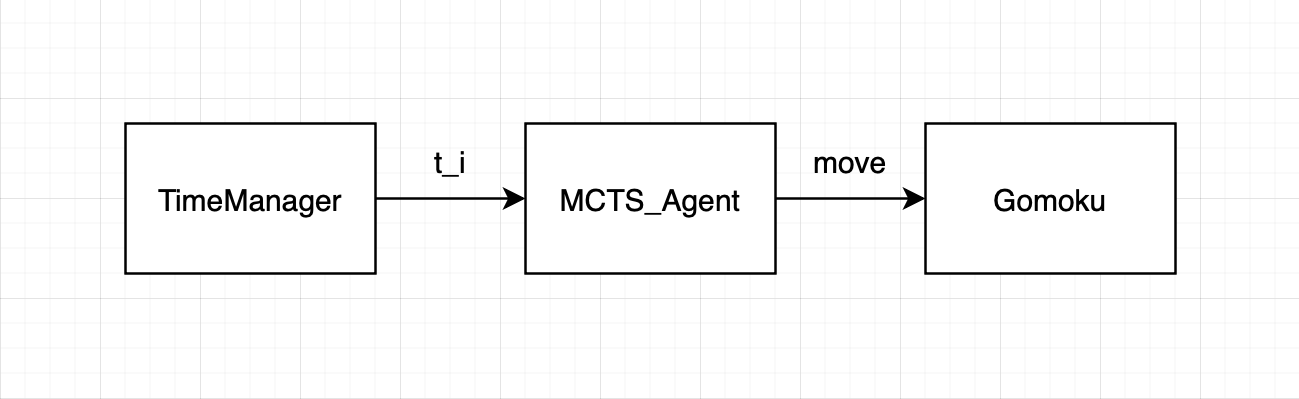
\includegraphics[width=0.8\textwidth]{images/conceptual_architecture.png}
    \caption{Arquitetura conceitual da solução. O gerenciador de tempo (\emph{TimeManager}) observa o estado da partida e determina o prazo $t_i$; o agente MCTS opera exclusivamente dentro desse prazo, retornando o movimento mais visitado ao seu término.}
    \label{fig:architecture}
    \legend{Fonte: Elaborado pelo autor}
\end{figure}

\subsection{Taxonomia das políticas por informação utilizada}
\label{sec:policy_taxonomy}

Uma distinção fundamental entre as políticas propostas é o conjunto de informações que cada uma utiliza para calcular $t_i$. Do ponto de vista da observabilidade, as políticas podem ser classificadas em duas categorias:

\textbf{Políticas agnósticas ao tabuleiro} (\emph{open-loop}): dependem apenas de variáveis globais da partida — tempo restante $T_r$ e número do lance $i$ — sem examinar o estado atual do tabuleiro. Apenas a estratégia uniforme (flat) se enquadra estritamente nessa categoria. Ela é computacionalmente trivial e determinística dado o histórico de tempo consumido; sua limitação é justamente a indiferença ao conteúdo posicional da partida.

\textbf{Políticas sensíveis ao tabuleiro} (\emph{closed-loop}): examinam o estado atual do tabuleiro para calibrar a alocação. A estratégia proporcional lê a contagem agregada de células vazias para computar a fração de preenchimento; a estratégia por fase classifica essa fração em regiões de importância distinta; a estratégia crítica inspeciona padrões táticos específicos. Essas políticas têm potencialmente maior poder de discriminação — alocam mais tempo precisamente quando o tabuleiro indica que o lance é importante —, mas introduzem um custo de análise do estado que deve ser negligenciável em relação a $t_i$ para não distorcer o experimento.

Entre as estratégias \emph{closed-loop}, o grau de sofisticação da informação extraída cresce da proporcional (contagem agregada) para a por fase (classificação ordinal) e a crítica (detecção de padrões posicionais específicos).

\subsection{Requisitos da interface de alocação}
\label{sec:interface_requirements}

Para que a separação entre política e motor de busca seja válida experimentalmente, a interface de alocação deve satisfazer dois requisitos. Primeiro, a política não pode modificar nem consultar o estado interno da árvore MCTS: toda informação que a política utiliza deve ser derivável do estado público da partida (tabuleiro, contadores de tempo, número do lance). Segundo, a política deve ser computacionalmente barata: seu tempo de execução deve ser ordens de grandeza inferior a $t_i$, de modo que a decisão de alocação em si não consuma orçamento significativo.

Esses requisitos garantem que, em todos os experimentos, o motor MCTS subjacente seja idêntico e que o único fator variado seja a distribuição de tempo entre os lances — condição necessária para atribuir diferenças de desempenho à estratégia de tempo e não a artefatos de implementação.

% ---
\section{Estratégias Propostas}
\label{sec:strategies}

As quatro estratégias a seguir derivam diretamente dos tipos de alocação catalogados na Seção~\ref{sec:timealloc_types} e das propriedades do Gomoku descritas na Seção~\ref{sec:gomoku_mcts}. Cada estratégia é apresentada com sua motivação e a hipótese de ganho que ela pretende explorar.

\subsection{Uniforme (\emph{Flat})}
\label{sec:strategy_flat}

A estratégia uniforme divide o orçamento restante pelo número estimado de movimentos restantes (Equação~\ref{eq:flat}):

\begin{equation}
    t_i = \frac{T_r}{\hat{N}_r}
\label{eq:flat}
\end{equation}

onde $T_r$ é o tempo restante e $\hat{N}_r$ é a estimativa do número de movimentos que o jogador ainda realizará na partida. Essa estratégia não distingue entre fases ou posições: trata todos os lances como igualmente valiosos. Ela serve como \emph{baseline} natural — qualquer estratégia mais sofisticada deve superá-la para justificar sua complexidade adicional. Sua previsibilidade é também uma vantagem prática: o agente nunca esgota prematuramente seu orçamento.

\subsection{Proporcional}
\label{sec:strategy_proportional}

A estratégia proporcional mantém a mesma forma da Equação~\ref{eq:flat}, mas aplica um multiplicador $\mu_{\text{prop}}$ que escala linearmente com o preenchimento do tabuleiro $\rho$:

\begin{equation}
    \rho = 1 - \frac{|\text{células vazias}|}{15^2}, \qquad
    \mu_{\text{prop}} = 0{,}8 + 0{,}4 \cdot \rho
\label{eq:prop_preview}
\end{equation}

Lances iniciais, com tabuleiro esparso, recebem ligeiramente menos tempo que a estratégia uniforme ($0{,}8\times$), enquanto lances tardios, com o tabuleiro mais preenchido, recebem mais ($1{,}2\times$). O multiplicador cresce linearmente com o preenchimento, mantendo o orçamento global próximo à estratégia uniforme em média. A hipótese é que lances tardios — com fator de ramificação menor e posições mais definidas — se beneficiam de mais tempo, ao passo que lances de abertura, com espaço de busca enorme e pouco retorno marginal por iteração adicional, podem ser resolvidos com menos tempo.

\subsection{Por Fase (\emph{Phase})}
\label{sec:strategy_phase}

A estratégia por fase classifica o estado da partida em fases — abertura, meio do jogo e final — e aplica um multiplicador distinto sobre a alocação uniforme em cada fase (Equação~\ref{eq:phase}):

\begin{equation}
    t_i = \mu_{\text{fase}} \cdot \frac{T_r}{\hat{N}_r}
\label{eq:phase}
\end{equation}

Os multiplicadores partem de uma hipótese de design: investir mais tempo nas fases iniciais da partida reduz a probabilidade de o agente se colocar em posições estruturalmente desfavoráveis, enquanto o meio do jogo — fase de maior complexidade tática — concentra as decisões que determinam o resultado. Sob essa hipótese, a abertura recebe um leve bônus ($\mu_{\text{abertura}} = 1{,}20$) para que o MCTS construa estimativas iniciais razoáveis em um tabuleiro ainda esparso e de ramificação máxima; o meio do jogo recebe o maior bônus ($\mu_{\text{meio}} = 1{,}50$) pela densidade de ameaças táticas que emergem nessa fase; e o final recebe desconto ($\mu_{\text{final}} = 0{,}55$) tanto pela hipótese de que o tabuleiro mais preenchido facilita a busca quanto pela necessidade de compensar os gastos extras das fases anteriores. Esses valores não derivam de uma caracterização formal do Gomoku, mas de uma intuição sobre a estrutura típica de uma partida — o que os torna suscetíveis à miscalibração, como os resultados experimentais confirmam.

\subsection{Crítica (\emph{Critical})}
\label{sec:strategy_critical}

A estratégia crítica opera no nível do lance individual: a cada turno, avalia se existe uma ameaça tática imediata no estado atual do tabuleiro. Na presença de uma ameaça — definida aqui como uma sequência de quatro peças em linha de qualquer jogador com ao menos uma extremidade aberta — o tempo alocado é multiplicado por um fator $\mu_{\text{crit}} > 1$; caso contrário, aplica-se um desconto $\mu_{\text{normal}} < 1$ para manter o orçamento equilibrado ao longo da partida (Equação~\ref{eq:critical}):

\begin{equation}
    t_i =
    \begin{cases}
        \mu_{\text{crit}} \cdot \dfrac{T_r}{\hat{N}_r}    & \text{se há ameaça tática detectada}  \\[6pt]
        \mu_{\text{normal}} \cdot \dfrac{T_r}{\hat{N}_r}  & \text{caso contrário}
    \end{cases}
\label{eq:critical}
\end{equation}

A hipótese central dessa estratégia é que erros em posições com ameaça de 4-em-linha aberta são imediatamente fatais: o agente que não bloqueia ou não completa a sequência perde a partida no lance seguinte. Nessas posições, investir tempo adicional tem retorno esperado muito superior à média, pois reduz diretamente a probabilidade de um erro irreparável. A detecção de ameaças funciona como um sinal de alta informatividade que o agente usa para redistribuir o orçamento de forma reativa.

A escolha do 4-em-linha aberto como sinal de detecção — em detrimento de outros padrões táticos relevantes no Gomoku, como o duplo-três — baseia-se em dois critérios. Primeiro, \textbf{imediaticidade}: uma ameaça de 4-em-linha aberta exige resposta obrigatória no lance imediatamente seguinte; ignorá-la resulta em derrota certa, tornando a posição inequivocamente crítica. O duplo-três, embora force vitória a médio prazo, oferece ao oponente ao menos um lance adicional de resposta, tornando sua criticidade menos imediata e o sinal menos preciso. Segundo, \textbf{simplicidade da política}: o objetivo desta estratégia não é construir um detector tático completo, mas sim avaliar se um sinal posicional simples e de alta precisão é suficiente para produzir ganho mensurável em taxa de vitórias. Ampliar a detecção para padrões adicionais aumentaria a complexidade da política sem isolar o efeito do sinal escolhido — dificultando a interpretação dos resultados. A extensão da detecção para padrões como o duplo-três permanece como direção natural de trabalho futuro (Seção~\ref{sec:discussion_limitations}).

\subsection{Comparação entre as estratégias}
\label{sec:strategies_comparison}

As quatro estratégias podem ser situadas ao longo de três dimensões: (i) a informação utilizada para calcular $t_i$; (ii) o mecanismo pelo qual redistribuem o orçamento; e (iii) o cenário de partida em que se espera que a redistribuição traga ganho.

A Tabela~\ref{tab:strategies_comparison} sumariza essas dimensões. A estratégia uniforme (\emph{open-loop}) usa estimador constante $\hat{N}_r$ e não consulta o tabuleiro. As estratégias \emph{closed-loop} (proporcional, por fase e crítica) complementam o mesmo estimador com informação do tabuleiro em graus crescentes de sofisticação: a proporcional extrai apenas a contagem agregada de peças (fração de preenchimento), a por fase classifica o estado em regiões de importância média distinta, e a crítica reage a eventos posicionais específicos de alta importância pontual.

\begin{table}[htbp]
    \centering
    \caption{Comparação das estratégias de alocação de tempo propostas.}
    \label{tab:strategies_comparison}
    \begin{tabular}{lllp{5cm}}
        \hline
        \textbf{Estratégia} & \textbf{Tipo} & \textbf{Sinal utilizado} & \textbf{Cenário de ganho esperado} \\
        \hline
        Uniforme    & Open-loop   & Tempo restante           & Baseline; sem cenário de ganho específico \\
        Proporcional & Closed-loop & Fração de preenchimento  & Lances tardios com menor fator de ramificação \\
        Por Fase    & Closed-loop & Fase do jogo             & Meio do jogo denso em ameaças táticas \\
        Crítica     & Closed-loop & Ameaças de 4-em-linha    & Posições com ameaça tática imediata \\
        \hline
    \end{tabular}
\end{table}

Do ponto de vista de risco orçamentário, a estratégia uniforme é a mais conservadora: aloca exatamente $T_r / \hat{N}_r$ por lance. A proporcional varia entre $0{,}8$ e $1{,}2$ vezes esse valor, mantendo o orçamento global próximo à uniforme em média. As estratégias por fase e crítica introduzem multiplicadores mais amplos (até $1{,}5\times$ e $2{,}0\times$, respectivamente) que podem consumir uma fração desproporcional do orçamento se ativados frequentemente — o que motiva a inclusão de fatores de desconto ($\mu < 1$) nos lances não críticos para manter o balanço orçamentário ao longo da partida. A Figura~\ref{fig:time_profiles} ilustra o perfil de alocação de cada estratégia ao longo de uma partida representativa.

A Tabela~\ref{tab:parameters} centraliza todos os parâmetros numéricos das estratégias, com os valores utilizados nos experimentos e a motivação para cada escolha.

\begin{table}[htbp]
    \centering
    \caption{Parâmetros das estratégias de alocação de tempo e valores utilizados nos experimentos.}
    \label{tab:parameters}
    \begin{tabular}{llrp{5.5cm}}
        \hline
        \textbf{Estratégia} & \textbf{Parâmetro} & \textbf{Valor} & \textbf{Motivação} \\
        \hline
        Todas       & $N_{\text{const}}$         & 75       & Margem acima da duração média observada (52 lances/jogador) \\
        \hline
        Proporcional & $\mu_{\text{min}}$         & 0,80     & Desconto na abertura (tabuleiro esparso) \\
                    & $\mu_{\text{max}}$         & 1,20     & Bônus no final (menor ramificação) \\
        \hline
        Por Fase    & $\mu_{\text{abertura}}$    & 1,20     & Leve bônus para evitar erros posicionais iniciais \\
                    & $\mu_{\text{meio}}$        & 1,50     & Fase com maior densidade de ameaças táticas \\
                    & $\mu_{\text{final}}$       & 0,55     & Desconto para compensar gasto extra nas fases anteriores \\
                    & Limiar abertura/meio       & $p = 0{,}10$ & Primeiros $\approx$10\% de preenchimento ($\approx$12 lances) \\
                    & Limiar meio/final          & $p = 0{,}45$ & Próximo ao preenchimento máximo observado na maioria das partidas \\
        \hline
        Crítica     & $\mu_{\text{crit}}$        & 2,00     & Dobrar o tempo em posições forçadas \\
                    & $\mu_{\text{normal}}$      & 0,90     & Desconto leve para compensar os picos críticos \\
        \hline
    \end{tabular}
\end{table}

\begin{figure}[htbp]
    \centering
    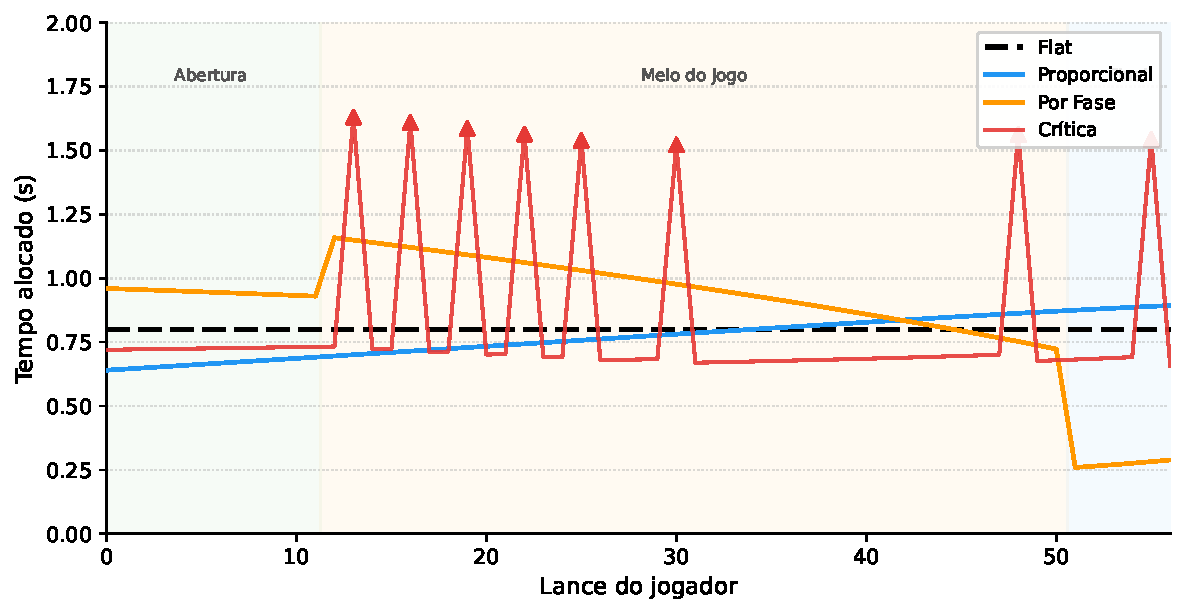
\includegraphics[width=0.8\textwidth]{images/time_profiles}
    \caption{Perfil conceitual de tempo alocado por lance ao longo de uma partida para cada uma das quatro estratégias. A estratégia uniforme produz uma linha aproximadamente horizontal; a proporcional cresce suavemente; a por fase exibe um platô elevado no meio do jogo; a crítica apresenta picos nos lances em que ameaças táticas são detectadas.}
    \label{fig:time_profiles}
    \legend{Fonte: Elaborado pelo autor}
\end{figure}

Uma limitação comum a todas as estratégias é que nenhuma delas considera o estado interno da árvore MCTS — por exemplo, a variância nas estimativas de valor dos filhos da raiz — como sinal de alocação. Abordagens que utilizam essa informação, como a proposta por \citet{huang2010time}, podem identificar posições de alta incerteza independentemente da fase ou de padrões táticos específicos. Essas abordagens estão fora do escopo deste trabalho, mas constituem uma extensão natural e são retomadas na Seção de trabalhos futuros.

% -----------------------------------------------------------------------
% CAPÍTULO 4 — Implementação
% -----------------------------------------------------------------------
\chapter{Implementação}
\label{chap:implementation}

Este capítulo descreve a implementação do sistema desenvolvido para este trabalho. A Seção~\ref{sec:impl_overview} apresenta a visão geral da arquitetura de módulos. A Seção~\ref{sec:impl_game} descreve o motor de jogo Gomoku. A Seção~\ref{sec:impl_mcts} detalha o agente MCTS. A Seção~\ref{sec:impl_timemanager} documenta a camada de gerenciamento de tempo e os parâmetros específicos de cada estratégia. A Seção~\ref{sec:impl_runner} descreve o \emph{runner} de torneio utilizado nos experimentos.

% ---
\section{Visão Geral do Sistema}
\label{sec:impl_overview}

O sistema é organizado em quatro módulos independentes que se comunicam por interfaces bem definidas (Figura~\ref{fig:modules}). O módulo \texttt{game/gomoku} implementa as regras e a representação de estados do Gomoku. O módulo \texttt{agents/mcts} implementa o agente de busca. O módulo \texttt{time\_manager} implementa as políticas de alocação de tempo. Um script \texttt{run\_duel.py} orquestra os duelos e coleta métricas. A estrutura de diretórios \texttt{game/} e \texttt{agents/} foi concebida de forma extensível: novos domínios de jogo ou novos agentes de busca podem ser integrados sem alterações na camada de gerenciamento de tempo ou no runner, embora neste trabalho apenas Gomoku e MCTS sejam instanciados.

\begin{figure}[htbp]
    \centering
    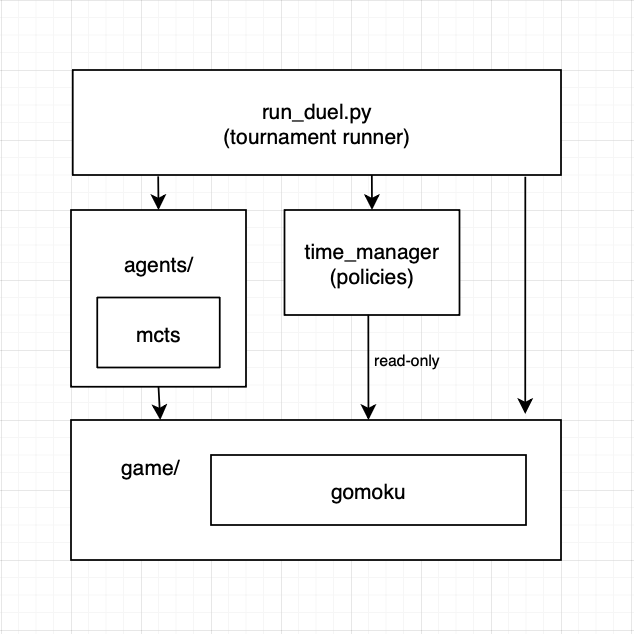
\includegraphics[width=0.8\textwidth]{images/modules_diagram.png}
    \caption{Diagrama de módulos do sistema. As setas indicam dependências: \texttt{run\_duel.py} consome os três módulos inferiores; \texttt{agents/mcts} consome \texttt{game/gomoku}; \texttt{time\_manager} depende apenas de \texttt{game/gomoku} para leitura do estado do tabuleiro.}
    \label{fig:modules}
    \legend{Fonte: Elaborado pelo autor}
\end{figure}

A separação entre \texttt{agents/mcts} e \texttt{time\_manager} é o ponto central da arquitetura: o agente recebe apenas um prazo em segundos e desconhece qual política de tempo o gerou. Isso garante que os experimentos comparem exclusivamente o efeito da estratégia de alocação, mantendo o motor de busca idêntico em todos os duelos.

% ---
\section{Motor de Jogo}
\label{sec:impl_game}

\subsection{Tabuleiro (\texttt{Board})}
\label{sec:impl_board}

O tabuleiro é representado por uma matriz $15 \times 15$ de caracteres: \texttt{'B'} para peça preta, \texttt{'W'} para peça branca e \texttt{'.'} para célula vazia. A interface pública relevante para este trabalho compreende:

\begin{itemize}
    \item \texttt{place\_marker(player, row, col)}: registra uma peça e atualiza o atributo \texttt{last\_move = (row, col, player)}, usado pelo \emph{rollout} do MCTS.
    \item \texttt{legal\_moves()}: retorna o conjunto de todas as células vazias como tuplas \texttt{(col, row)}.
    \item \texttt{is\_terminal\_state()}: retorna verdadeiro se algum jogador completou cinco em linha ou se o tabuleiro está completamente preenchido.
    \item \texttt{winner()}: retorna \texttt{'B'}, \texttt{'W'} ou \texttt{None} (empate).
\end{itemize}

\subsection{Estado de Jogo (\texttt{GameState})}
\label{sec:impl_gamestate}

\texttt{GameState} encapsula um \texttt{Board} e o jogador que deve mover. Suas operações principais são \texttt{next\_state(move)}, que cria uma cópia do estado com a peça posicionada e o jogador alternado, e \texttt{get\_board()}, que expõe o tabuleiro para as políticas de tempo. Todos os estados são imutáveis do ponto de vista do MCTS: cada expansão gera um novo objeto \texttt{GameState} sem modificar o estado pai.

% ---
\section{Agente MCTS}
\label{sec:impl_mcts}

\subsection{Loop principal baseado em tempo}
\label{sec:impl_mcts_loop}

A função \texttt{mcts\_search(root\_state, time\_limit)} recebe o estado raiz e o prazo em segundos. Internamente, converte o prazo em um \emph{deadline} absoluto e executa iterações enquanto o relógio não o ultrapassa:

\begin{equation}
    \text{deadline} = t_{\text{atual}} + t_i, \qquad
    \text{loop enquanto } t_{\text{atual}} < \text{deadline}
\label{eq:mcts_deadline}
\end{equation}

Cada iteração aplica as quatro fases do MCTS em sequência: seleção via UCT, expansão de um filho não visitado, simulação (\emph{rollout}) e retropropagação. Ao término do prazo, o algoritmo retorna o filho da raiz com maior contagem de visitas $N(v)$.

O uso do tempo como critério de parada — em vez de um número fixo de iterações — é o que torna o sistema diretamente controlável pelas políticas de tempo: cada estratégia determina $t_i$ e o MCTS realiza o máximo de iterações possível dentro desse orçamento. O número de iterações efetivamente realizadas é uma variável observada, não controlada.

\subsection{Seleção e UCT}
\label{sec:impl_uct}

Durante a fase de seleção, o algoritmo desce a árvore escolhendo em cada nó o filho que maximiza o critério UCB1 (Equação~\ref{eq:ucb1}) com constante $C = \sqrt{2}$. Nós não visitados ($N(v) = 0$) são priorizados imediatamente, garantindo que todos os filhos sejam amostrados ao menos uma vez antes de qualquer seleção por UCT.

\subsection{Rollout com viés de localidade}
\label{sec:impl_rollout}

O \emph{rollout} simula uma partida a partir do nó expandido até um estado terminal ou até o limite de 200 movimentos. Em vez de escolher movimentos uniformemente ao acaso, o \emph{rollout} adota um viés de localidade: prefere movimentos dentro de um raio $r = 5$ ao redor da última peça colocada no tabuleiro. Formalmente, dada a última peça em $(r_{\text{last}}, c_{\text{last}})$, o conjunto preferencial de movimentos é:

\begin{equation}
    A_{\text{local}} = \left\{ (x, y) \in A \;\middle|\; |y - r_{\text{last}}| \leq 5 \;\text{ e }\; |x - c_{\text{last}}| \leq 5 \right\}
\label{eq:locality_bias}
\end{equation}

Se $A_{\text{local}} \neq \emptyset$, o \emph{rollout} escolhe uniformemente em $A_{\text{local}}$; caso contrário, escolhe em $A$ inteiro. Esse viés reduz efetivamente o espaço de busca durante a simulação — movimentos distantes de qualquer peça são raramente relevantes no Gomoku — e acelera a convergência das estimativas de valor sem requerer uma função de avaliação heurística.

\subsection{Retropropagação}
\label{sec:impl_backprop}

A retropropagação percorre o caminho da folha até a raiz de forma iterativa. O resultado do \emph{rollout} ($1{,}0$ para vitória, $0{,}0$ para derrota, $0{,}5$ para empate) é invertido a cada nível — $\text{resultado} \leftarrow 1{,}0 - \text{resultado}$ — para refletir a alternância de perspectivas entre jogadores consecutivos na árvore.

% ---
\section{Camada de Gerenciamento de Tempo}
\label{sec:impl_timemanager}

\subsection{Interface \texttt{BaseTimeManager}}
\label{sec:impl_base}

Todas as estratégias implementam o método abstrato:

\begin{center}
\texttt{allocate(time\_remaining, move\_number, board, player) -> float}
\end{center}

O valor retornado é então limitado pelo \emph{runner} ao intervalo efetivo:

\begin{equation}
    t_i^{\text{eff}} = \max\!\bigl(0{,}05,\; \min(t_i,\; T_r \cdot 0{,}95)\bigr)
\label{eq:clamp}
\end{equation}

O limite inferior de $0{,}05$ s garante ao menos uma iteração MCTS; o limite superior de $95\%$ do tempo restante previne que um único lance esgote o orçamento. O método \texttt{clamp} da classe base aplica o limite inferior; o limite de $95\%$ é aplicado em \texttt{run\_duel.py} após o retorno da política.

\subsection{Estratégia Flat}
\label{sec:impl_flat}

A estratégia uniforme usa um estimador constante do número de movimentos restantes (Equação~\ref{eq:flat_impl}):

\begin{equation}
    \hat{N}_r = \max\!\bigl(1,\; N_{\text{const}} - i\bigr), \qquad N_{\text{const}} = 75
\label{eq:flat_impl}
\end{equation}

onde $i$ é o número de movimentos já realizados pelo jogador. O valor $N_{\text{const}} = 75$ foi calibrado empiricamente a partir das partidas observadas: a duração média foi de $52{,}2$ lances por jogador (mediana 54, máximo observado 76). O valor 75 mantém uma margem de segurança para partidas acima da média sem supralocar orçamento nos lances iniciais.

\subsection{Estratégia Proporcional}
\label{sec:impl_proportional}

A estratégia proporcional utiliza o mesmo estimador $\hat{N}_r$ da estratégia uniforme, mas aplica um multiplicador que escala linearmente com o preenchimento do tabuleiro (Equação~\ref{eq:proportional_impl}):

\begin{equation}
    \rho = 1 - \frac{|\text{células vazias}|}{15^2}, \qquad
    \mu_{\text{prop}} = 0{,}8 + 0{,}4 \cdot \rho
\label{eq:proportional_impl}
\end{equation}

O tempo alocado ao lance é então:

\begin{equation}
    t_i = \mu_{\text{prop}} \cdot \frac{T_r}{\hat{N}_r}
\end{equation}

Com tabuleiro vazio ($\rho = 0$), o multiplicador vale $0{,}8$ — ligeiramente abaixo da uniforme. À medida que o tabuleiro enche, o multiplicador cresce linearmente até $1{,}2$ quando o tabuleiro está completamente preenchido. Como a maioria das partidas termina com preenchimento entre 20\% e 60\%, o multiplicador médio efetivo permanece próximo de $1{,}0$, mantendo o orçamento global equivalente à uniforme enquanto redistribui tempo dos lances iniciais para os lances finais.

\subsection{Estratégia por Fase}
\label{sec:impl_phase}

A estratégia por fase utiliza o mesmo $\hat{N}_r$ da estratégia uniforme e determina a fase do jogo pela fração de preenchimento do tabuleiro (Equação~\ref{eq:fill_progress}):

\begin{equation}
    p = 1 - \frac{|\text{células vazias}|}{15^2}
\label{eq:fill_progress}
\end{equation}

A partir de $p$, a fase é determinada por limiares fixos:

\begin{equation}
    \text{fase}(p) =
    \begin{cases}
        \text{abertura}       & \text{se } p < 0{,}10 \\
        \text{meio do jogo}   & \text{se } 0{,}10 \leq p < 0{,}45 \\
        \text{final}          & \text{se } p \geq 0{,}45
    \end{cases}
\end{equation}

Os multiplicadores aplicados sobre $T_r / \hat{N}_r$ são $\mu_{\text{abertura}} = 1{,}20$, $\mu_{\text{meio}} = 1{,}50$ e $\mu_{\text{final}} = 0{,}55$. Os limiares foram calibrados empiricamente: a abertura cobre os primeiros $\approx 10\%$ de preenchimento (cerca de 12 lances por jogador), o meio do jogo estende-se até $45\%$ de preenchimento — valor próximo ao limite máximo observado na maioria das partidas — e o final cobre o restante. O multiplicador reduzido no final ($0{,}55$) compensa o orçamento extra destinado às fases anteriores, mantendo o balanço global próximo à uniforme.

\subsection{Estratégia Crítica}
\label{sec:impl_critical}

A estratégia crítica utiliza o mesmo $\hat{N}_r$ da estratégia uniforme e detecta ameaças de 4-em-linha com ao menos uma extremidade aberta para qualquer um dos dois jogadores. A detecção percorre as quatro direções (horizontal, vertical, diagonal principal, diagonal secundária) e verifica, para cada sequência de comprimento $\geq 4$, se a célula imediatamente anterior ou posterior está vazia (Equação~\ref{eq:critical_impl}):

\begin{equation}
    t_i =
    \begin{cases}
        2{,}0 \cdot \dfrac{T_r}{\hat{N}_r} & \text{se ameaça de 4-em-linha detectada} \\[6pt]
        0{,}9 \cdot \dfrac{T_r}{\hat{N}_r} & \text{caso contrário}
    \end{cases}
\label{eq:critical_impl}
\end{equation}

O fator de desconto $0{,}9$ nos lances não críticos compensa o orçamento extra consumido nas posições críticas, mantendo o balanço total próximo ao da estratégia uniforme ao longo de uma partida típica.

% ---
\section{Runner de Torneio}
\label{sec:impl_runner}

O script \texttt{run\_duel.py} executa $N$ partidas entre dois agentes MCTS com estratégias de tempo distintas. Para controlar o viés do primeiro movimento, as cores são alternadas a cada partida: na partida par, a estratégia em avaliação joga com as peças pretas; na partida ímpar, joga com as brancas.

A cada lance, o \emph{runner} registra quatro métricas: tempo alocado pela política ($t_i^{\text{eff}}$), tempo efetivamente consumido pelo MCTS, tempo restante após o lance e o movimento escolhido. Ao final de todas as partidas, os resultados são serializados em JSON com três seções:

\begin{itemize}
    \item \texttt{config}: todos os parâmetros da execução (estratégias, orçamento, número de partidas), garantindo reprodutibilidade.
    \item \texttt{summary}: taxa de vitórias agregada e por cor para cada estratégia, tempo médio alocado por lance.
    \item \texttt{matches}: lista completa de partidas com o log de movimentos por lance.
\end{itemize}

Essa estrutura permite tanto a análise agregada de taxa de vitórias (Capítulo~\ref{chap:results}) quanto a análise temporal da distribuição de tempo ao longo das partidas.

% -----------------------------------------------------------------------
% CAPÍTULO 5 — Resultados e Análise
% -----------------------------------------------------------------------
\chapter{Resultados e Análise}
\label{chap:results}

Este capítulo apresenta e analisa os resultados dos experimentos de torneio descritos na Seção~\ref{sec:impl_runner}. A Seção~\ref{sec:exp_setup} descreve a configuração experimental e a metodologia estatística adotada. A Seção~\ref{sec:results_overview} apresenta uma visão geral dos resultados. A Seção~\ref{sec:results_per_strategy} analisa cada estratégia individualmente. A Seção~\ref{sec:results_discussion} discute os achados em conjunto e os situa no contexto das hipóteses propostas no Capítulo~\ref{chap:proposal}.

% ---
\section{Configuração Experimental}
\label{sec:exp_setup}

Cada estratégia foi avaliada em torneios de $N = 400$ partidas contra o \emph{baseline} uniforme em três orçamentos de tempo distintos: 30, 60 e 120 segundos por jogador por partida. Para controlar o viés do primeiro movimento — Preto possui vantagem estrutural em Gomoku, conforme discutido na Seção~\ref{sec:gomoku_rules} — as 400 partidas de cada configuração foram divididas igualmente entre as duas cores: 200 partidas com a estratégia em avaliação jogando como Preto e 200 como Branco. O orçamento de 60 segundos constitui o experimento principal; os orçamentos de 30 e 120 segundos foram conduzidos para avaliar a robustez dos resultados a variações no recurso computacional disponível. No total, foram realizadas 3600 partidas de torneio.

\textbf{Metodologia estatística.} O resultado de cada partida é modelado como uma variável de Bernoulli: vitória (1) ou derrota (0). Para cada estratégia, estimou-se a taxa de vitórias $\hat{p} = w / N$ e construiu-se um intervalo de confiança de 95\% pela aproximação normal:

\begin{equation}
    \text{IC}_{95\%} = \hat{p} \pm 1{,}96 \sqrt{\frac{\hat{p}(1-\hat{p})}{N}}
\label{eq:ci}
\end{equation}

A hipótese nula $H_0\colon p = 0{,}5$ — a estratégia tem a mesma taxa de vitórias que o \emph{baseline} — foi testada pelo escore $z$:

\begin{equation}
    z = \frac{\hat{p} - 0{,}5}{\sqrt{0{,}25/N}}
\label{eq:ztest}
\end{equation}

Não foram observados empates em nenhuma das 3600 partidas realizadas, o que é consistente com a propriedade do Gomoku de que o jogo ótimo resulta sempre em vitória do primeiro jogador \cite{allis1994searching}.

% ---
\section{Visão Geral dos Resultados}
\label{sec:results_overview}

A Tabela~\ref{tab:results_main} apresenta as taxas de vitórias de cada estratégia no experimento principal (60 segundos), desagregadas por cor e no total, com os respectivos intervalos de confiança e estatísticas de teste.

\begin{table}[htbp]
    \centering
    \caption{Taxas de vitórias das estratégias contra o \emph{baseline} uniforme, experimento principal com orçamento de 60 s ($N = 400$ partidas por estratégia, 200 por cor). IC: intervalo de confiança de 95\%. Significância: *** $p < 0{,}001$, ** $p < 0{,}01$, n.s.\ não significativo.}
    \label{tab:results_main}
    \begin{tabular}{llrrrlr}
        \hline
        \textbf{Estratégia} & \textbf{Cor} & \textbf{Vitórias} & \textbf{Partidas} & \textbf{Taxa} & \textbf{IC 95\%} & \textbf{Sig.} \\
        \hline
        Crítica      & Preto & 123 & 200 & 61,5\% & [54,8\%; 68,2\%] & **  \\
                     & Branco & 124 & 200 & 62,0\% & [55,3\%; 68,7\%] & *** \\
                     & Total & 247 & 400 & \textbf{61,8\%} & [57,0\%; 66,5\%] & *** \\
        \hline
        Por Fase     & Preto &  89 & 200 & 44,5\% & [37,6\%; 51,4\%] & n.s.\\
                     & Branco &  72 & 200 & 36,0\% & [29,3\%; 42,7\%] & *** \\
                     & Total & 161 & 400 & \textbf{40,2\%} & [35,4\%; 45,1\%] & *** \\
        \hline
        Proporcional & Preto & 103 & 200 & 51,5\% & [44,6\%; 58,4\%] & n.s.\\
                     & Branco & 106 & 200 & 53,0\% & [46,1\%; 59,9\%] & n.s.\\
                     & Total & 209 & 400 & \textbf{52,2\%} & [47,4\%; 57,1\%] & n.s.\\
        \hline
    \end{tabular}
\end{table}

Os resultados dividem-se em três categorias distintas: a estratégia crítica supera significativamente o \emph{baseline}; a estratégia por fase é significativamente inferior; e a estratégia proporcional é indistinguível do \emph{baseline}. A Figura~\ref{fig:results_winrates} ilustra essa comparação visualmente.

A Tabela~\ref{tab:results_budgets} resume os resultados dos três orçamentos testados, possibilitando avaliar a robustez de cada estratégia.

\begin{table}[htbp]
    \centering
    \caption{Taxas de vitórias totais por estratégia e orçamento de tempo ($N = 400$ partidas por célula). Significância: *** $p < 0{,}001$, ** $p < 0{,}01$, * $p < 0{,}05$, n.s.\ não significativo.}
    \label{tab:results_budgets}
    \begin{tabular}{lrrr}
        \hline
        \textbf{Estratégia} & \textbf{30 s} & \textbf{60 s} & \textbf{120 s} \\
        \hline
        Crítica      & 51,0\% (n.s.) & \textbf{61,8\%} (***) & \textbf{63,2\%} (***) \\
        Por Fase     & 44,5\% (*)    & 40,2\% (***)          & 42,5\% (**)           \\
        Proporcional & 48,2\% (n.s.) & 52,2\% (n.s.)         & 50,5\% (n.s.)         \\
        \hline
    \end{tabular}
\end{table}

\begin{figure}[htbp]
    \centering
    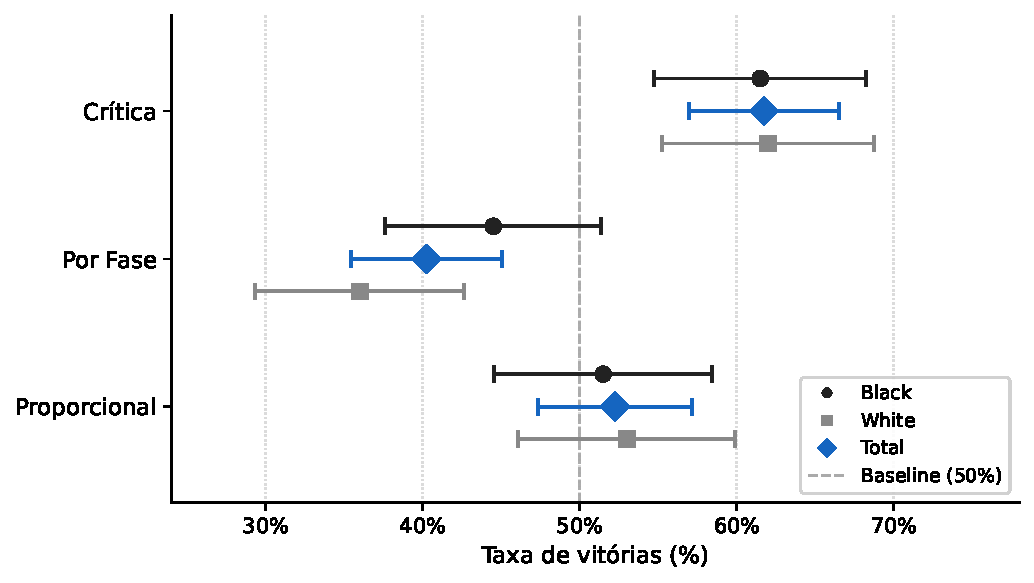
\includegraphics[width=0.85\textwidth]{images/results_winrates}
    \caption{Taxas de vitórias por estratégia e cor, com intervalos de confiança de 95\%. A linha tracejada em 50\% indica o nível do \emph{baseline} uniforme. A estratégia crítica supera consistentemente o \emph{baseline} em ambas as cores; a por fase fica consistentemente abaixo; a proporcional mantém-se próxima de 50\%.}
    \label{fig:results_winrates}
    \legend{Fonte: Elaborado pelo autor}
\end{figure}

% ---
\section{Análise por Estratégia}
\label{sec:results_per_strategy}

\subsection{Estratégia Crítica}
\label{sec:results_critical}

A estratégia crítica obteve 61,8\% de vitórias no total ($z = +4{,}70$, $p < 0{,}001$), resultado altamente significativo. O achado mais notável é a \textbf{simetria entre cores}: 61,5\% como Preto e 62,0\% como Branco, uma diferença de apenas 0,5 pontos percentuais. Em Gomoku, \citet{allis1994searching} provou que, com jogo ótimo, o primeiro jogador vence; contudo, no contexto deste experimento — com agentes MCTS de força equivalente — a partida de controle (uniforme vs.\ uniforme) resultou em 49,5\% de vitórias para Preto e 50,5\% para Branco, confirmando que os agentes não jogam de forma ótima e que a vantagem teórica do primeiro movimento não é observável neste nível de jogo. O fato de a estratégia crítica obter 62\% como Branco — jogando contra a estratégia uniforme como Preto — indica que a detecção de ameaças confere uma vantagem real, independente da cor.

A análise da distribuição de tempo revela que a estratégia crítica gastou em média 0,878 s/lance, contra 0,796 s/lance da uniforme — uma diferença de aproximadamente 10\%. Esse acréscimo não é uniforme: ameaças táticas foram detectadas em \textbf{20,4\% dos lances} (aproximadamente 1 em cada 5), nos quais o tempo alocado subiu para cerca de 1,4 s, enquanto os demais lances receberam $0{,}9\times$ da alocação uniforme. O sinal de detecção de ameaças é, portanto, esparso mas de alta precisão: identifica exatamente os lances em que um erro é imediatamente fatal e concentra recursos neles.

Esse resultado valida a hipótese central da estratégia crítica (Seção~\ref{sec:strategy_critical}): erros em posições com ameaça de 4-em-linha aberta têm custo irreparável, e investir tempo adicional nesses lances — ainda que em apenas 20\% dos casos — eleva significativamente a taxa de vitórias.

\textbf{Ganho de busca nos lances críticos.} Como o agente MCTS opera em modo \emph{CPU-bound} — executa iterações continuamente até o \emph{deadline} —, o tempo efetivamente consumido é proporcional ao número de iterações realizadas. Nos lances críticos, o tempo médio gasto foi de 1,42 s, contra 0,80 s do \emph{baseline} uniforme — uma razão de $1{,}76\times$, ou seja, aproximadamente 76\% mais iterações de busca exatamente nas posições com ameaça de 4-em-linha. Nos lances não críticos, o desconto de $0{,}9\times$ resultou em 0,75 s gastos, 7\% abaixo da uniforme. A estratégia crítica, portanto, não apenas realoca tempo no papel: ela entrega concretamente mais profundidade de busca nos gargalos táticos e levemente menos nos lances de baixa urgência.

\textbf{Robustez ao orçamento de tempo.} Os experimentos com 30, 60 e 120 segundos revelam um padrão de escalonamento positivo. Com 30 s, a estratégia crítica obtém 51,0\% ($z = +0{,}4$, n.s.): o ganho não é estatisticamente detectável com esse orçamento. Com 60 s, o ganho sobe para 61,8\% ($z = +4{,}70$, $p < 0{,}001$), e com 120 s atinge 63,2\% ($z = +5{,}30$, $p < 0{,}001$). Esse gradiente sugere que a estratégia crítica beneficia-se de orçamentos maiores: com mais tempo total disponível, o dobramento aplicado nos lances críticos representa um montante absoluto mais expressivo, permitindo ao MCTS explorar com maior profundidade justamente as posições forçadas. Com 30 s, o orçamento por lance é suficientemente pequeno para que mesmo o dobramento não garanta busca aprofundada suficiente; com 60 e 120 s, a concentração de recursos nos gargalos táticos se converte em ganho mensurável e crescente.

\subsection{Estratégia por Fase}
\label{sec:results_phase}

A estratégia por fase obteve 40,2\% de vitórias no total ($z = -3{,}90$, $p < 0{,}001$), sendo significativamente \emph{inferior} ao \emph{baseline}. O resultado é paradoxal à primeira vista: a estratégia por fase gastou em média 0,900 s/lance — 13\% a mais que a uniforme — e ainda assim obteve menor taxa de vitórias. O problema está na distribuição temporal, não no volume total.

A Tabela~\ref{tab:phase_time} mostra a alocação média por faixa de lances do jogador para a estratégia por fase e para a uniforme.

\begin{table}[htbp]
    \centering
    \caption{Tempo médio alocado por faixa de lance do jogador: estratégia por fase vs.\ uniforme (partidas como Preto, $n = 200$).}
    \label{tab:phase_time}
    \begin{tabular}{lrrr}
        \hline
        \textbf{Lances do jogador} & \textbf{Por Fase} & \textbf{Flat} & \textbf{Diferença} \\
        \hline
        0--10   (abertura)         & 0,946 s & 0,799 s & $+18\%$ \\
        11--25  (meio do jogo)     & 1,081 s & 0,797 s & $+36\%$ \\
        26--40  (meio/final)       & 0,938 s & 0,795 s & $+18\%$ \\
        41+     (final)            & 0,578 s & 0,791 s & $-27\%$ \\
        \hline
    \end{tabular}
\end{table}

O orçamento é gasto em excesso na abertura e no meio do jogo — fase em que o multiplicador de 1,5$\times$ eleva o gasto por lance em 36\% acima da uniforme — esgotando as reservas disponíveis para os lances finais. Quando o tabuleiro atinge o limiar de final ($p \geq 0{,}45$), dois efeitos negativos se combinam: (i) o orçamento residual já está reduzido pelo excesso de gastos anteriores, e (ii) o multiplicador de final ($\mu = 0{,}55$) desconta adicionalmente esse orçamento já reduzido. O resultado é que os lances 41+, onde as partidas costumaram ser decididas, recebem 27\% menos tempo que a uniforme.

A assimetria entre as cores reforça essa interpretação. Branco joga os lances de resposta em posições com tabuleiro mais preenchido, justamente quando o desconto de final está ativo. Isso explica a queda da taxa de vitórias de 44,5\% como Preto para 36,0\% como Branco.

O resultado aponta uma limitação de design: a hipótese motivadora da estratégia por fase — que o meio do jogo concentra as decisões mais consequentes — é plausível, mas o desconto de final de 0,55$\times$ acaba penalizando os lances decisivos em vez de preservar orçamento para eles. Um refinamento natural seria reduzir esse desconto ou substituir o limiar fixo de preenchimento pelo número de lances restantes estimados, desacoplando a classificação de fase do ritmo real de cada partida.

Há, porém, uma limitação mais profunda que vai além dos parâmetros escolhidos: \textbf{a fase do jogo é um indicador indireto fraco para a criticidade tática de um lance individual}. A estratégia por fase assume que a importância de um lance é determinada principalmente pela fase global da partida — abertura, meio do jogo ou final. Essa suposição ignora que a criticidade é essencialmente local: uma ameaça de 4-em-linha pode emergir no lance 8 (abertura) ou no lance 60 (final), independentemente do preenchimento médio do tabuleiro. Da mesma forma, muitos lances de meio do jogo são posicionais, sem ameaças táticas imediatas, e não se beneficiam de tempo adicional da mesma forma que uma posição forçada.

Em outras palavras, a estratégia por fase investe mais tempo nos lances do meio do jogo em média, mas sem discriminar quais lances do meio do jogo são genuinamente críticos. Ao redistribuir tempo de forma agregada por fase, ela inevitavelmente alocará mais tempo a lances de baixa urgência (e.g., jogadas posicionais de médio prazo) e, ao mesmo tempo, não garantirá recursos suficientes para lances críticos que ocorrem fora da janela de fase privilegiada. O contraste com a estratégia crítica é revelador: ao reagir ao estado local do tabuleiro em vez de à fase global, a estratégia crítica consegue concentrar o orçamento exatamente nos lances em que ele tem maior retorno esperado.

\textbf{Robustez ao orçamento de tempo.} Nos três orçamentos testados, a estratégia por fase é consistentemente inferior ao \emph{baseline}: 44,5\% com 30 s ($z = -2{,}2$, $p < 0{,}05$), 40,2\% com 60 s ($z = -3{,}9$, $p < 0{,}001$) e 42,5\% com 120 s ($z = -3{,}0$, $p < 0{,}01$). O efeito adverso é persistente e independente do orçamento, o que indica que o problema reside no design da estratégia — especificamente na miscalibração do desconto de final — e não num artefato específico ao orçamento de 60 segundos. Vale notar que com 120 s a penalização de Branco atenua-se ligeiramente (43,5\% vs.\ 36,0\% a 60 s), possivelmente porque o desconto por esgotamento antecipado de orçamento é menos severo quando o orçamento total é maior, mas o efeito ainda permanece significativamente negativo.

\subsection{Estratégia Proporcional}
\label{sec:results_proportional}

A estratégia proporcional obteve 52,2\% de vitórias no total ($z = +0{,}90$, $p = 0{,}37$), resultado estatisticamente indistinguível do \emph{baseline} com 400 partidas. A análise temporal revela que a estratégia proporcional gastou sistematicamente \textbf{menos} tempo que a uniforme: 0,758 s/lance contra 0,796 s/lance, uma redução de aproximadamente 5\%.

Essa subalocação ocorre porque a maioria dos lances se concentra nas fases iniciais da partida, quando o preenchimento do tabuleiro $\rho$ ainda é baixo. Com $\rho$ tipicamente entre 0\% e 30\% durante a maior parte da partida, o multiplicador $\mu = 0{,}8 + 0{,}4\rho$ oscila entre 0,80 e 0,92 — sistematicamente abaixo de 1,0. O acréscimo esperado nos lances finais ($\mu \to 1{,}2$) é parcialmente compensado pela redução do orçamento residual nesses lances.

A redistribuição de tempo é, portanto, mais tênue na prática do que na intenção de projeto, e seus efeitos não são detectáveis com 400 partidas. O resultado é neutro: a estratégia proporcional não prejudica nem beneficia o desempenho em relação à uniforme.

\textbf{Robustez ao orçamento de tempo.} O comportamento neutro mantém-se nos três orçamentos: 48,2\% com 30 s ($z = -0{,}7$, n.s.), 52,2\% com 60 s ($z = +0{,}9$, n.s.) e 50,5\% com 120 s ($z = +0{,}2$, n.s.). A ausência de efeito é consistente e independente do recurso computacional, reforçando que a estratégia proporcional, em sua forma atual, é equivalente ao \emph{baseline} uniforme em qualquer orçamento testado.

% ---
\section{Discussão}
\label{sec:results_discussion}

\subsection{Síntese comparativa}
\label{sec:discussion_synthesis}

Os três resultados formam um padrão coerente à luz das hipóteses do Capítulo~\ref{chap:proposal}. A estratégia com sinal de maior especificidade — a crítica, que detecta padrões posicionais concretos — é a única que produz ganho mensurável. A estratégia com sinal de especificidade intermediária — a por fase, que classifica o estado em regiões ordinais de importância — produz redistribuição de tempo mas com efeito adverso por conta da miscalibração do desconto de final. A estratégia com sinal mais fraco — a proporcional, com contagem agregada de peças — é neutra.

Esse gradiente sugere que, neste domínio e com este orçamento de tempo, \textbf{a qualidade do sinal de alocação importa mais do que o volume total de tempo redistribuído}. A estratégia crítica usa um sinal binário aplicado a aproximadamente 20\% dos lances — mecanismo simples, mas altamente informativo. A estratégia por fase distribui o orçamento de forma mais contínua mas com menor acurácia na identificação dos lances decisivos.

\subsection{Por que a estratégia crítica funciona}
\label{sec:discussion_critical}

O desempenho da estratégia crítica pode ser interpretado à luz de três conceitos complementares.

\textbf{Gargalos táticos e alocação seletiva de recursos.} Em jogos com ameaças forçadas, a qualidade da partida não é determinada pela média das decisões, mas pelos erros nos momentos de maior consequência. Um único lance mal respondido em uma posição de 4-em-linha aberta encerra a partida independentemente de quantas decisões anteriores foram de alta qualidade. Isso configura um gargalo tático: a distribuição de impacto dos lances é altamente assimétrica, com uma minoria de posições concentrando a maior parte do risco de derrota. A alocação seletiva de recursos — concentrar orçamento computacional nos gargalos — é precisamente o mecanismo que a estratégia crítica explora.

\textbf{Valor da informação e precisão do sinal.} Na perspectiva da teoria da decisão, o valor de investir tempo adicional em um lance é proporcional à probabilidade de que esse tempo altere a decisão tomada e ao impacto dessa mudança no resultado final. Em posições não críticas, o MCTS com orçamento uniforme já identifica o movimento correto com alta confiança — iterações adicionais têm baixo valor de informação. Em posições com ameaça de 4-em-linha, a probabilidade de erro sem tempo suficiente é não negligenciável, e o custo de um erro é máximo (derrota imediata). O sinal binário da estratégia crítica captura exatamente essa assimetria: ele não tenta estimar o valor de cada lance, apenas identifica quando o valor da informação adicional é excepcionalmente alto.

\textbf{Precisão versus cobertura do sinal.} A eficácia do sinal depende não apenas de detectar posições críticas, mas de não ativar o multiplicador em posições de baixa urgência. Um sinal de baixa precisão diluiria o orçamento extra e aproximaria a estratégia do comportamento da estratégia por fase. O 4-em-linha aberto é um sinal de alta precisão: cada ativação corresponde a uma posição genuinamente forçada. Isso explica por que uma taxa de ativação de apenas 20,4\% é suficiente para produzir ganho de 11,8 pontos percentuais — cada unidade de orçamento extra é investida exatamente onde tem maior retorno esperado.

\subsection{O efeito da cor na estratégia crítica}
\label{sec:discussion_color}

A simetria observada na estratégia crítica — 61,5\% como Preto e 62,0\% como Branco — merece atenção específica. A partida de controle (uniforme vs.\ uniforme a 60 s) produziu 49,5\% para Preto e 50,5\% para Branco, mostrando que, neste nível de jogo, os agentes MCTS de força equivalente não exibem a vantagem estrutural do primeiro movimento prevista pela análise de jogo ótimo \cite{allis1994searching}. Nesse contexto, a obtenção de 62\% como Branco pela estratégia crítica não representa reversão de uma desvantagem preexistente, mas sim uma vantagem real criada pela política de alocação: Branco, que tipicamente precisa reagir à iniciativa de Preto, se beneficia da detecção de ameaças porque bloquear uma sequência de 4-em-linha no tempo correto é, frequentemente, a única forma de não perder no lance seguinte.

\subsection{Limitações}
\label{sec:discussion_limitations}

Os experimentos apresentam algumas limitações que devem ser consideradas na interpretação dos resultados. Primeiro, o único \emph{baseline} utilizado foi a estratégia uniforme; comparações diretas entre as estratégias propostas não foram realizadas, o que impede afirmações sobre ordenação relativa entre elas. Segundo, embora os experimentos cubram três orçamentos distintos (30, 60 e 120 segundos), a estratégia crítica só apresenta ganho mensurável a partir de 60 s; o limiar mínimo de orçamento para que o mecanismo de detecção de ameaças produza efeito positivo não foi investigado sistematicamente. Terceiro, ambos os agentes utilizam o mesmo motor MCTS; contra agentes com capacidades de busca diferentes, os efeitos das estratégias de tempo podem variar. Por fim, os resultados são específicos ao Gomoku; domínios com estrutura tática distinta podem apresentar padrões diferentes de resposta às estratégias de alocação. Uma direção natural de trabalho futuro é estender o sistema a outros jogos de tabuleiro — como Go ou Hex — e a outros agentes de busca, explorando se o ganho da estratégia crítica se generaliza para domínios com padrões táticos diferentes, e se a arquitetura extensível proposta facilita essa comparação.

Uma limitação de design merece destaque adicional. O experimento não separa dois efeitos que a estratégia crítica combina: (i) redistribuição de volume — alocar mais tempo em um subconjunto de lances — e (ii) qualidade do sinal — escolher corretamente quais lances merecem mais tempo. O ganho observado pode resultar de qualquer combinação dos dois. O argumento comparativo disponível nos dados é sugestivo: a estratégia por fase redistribui 13\% mais tempo que a uniforme e perde; a proporcional redistribui e é neutra; a crítica redistribui 10\% a mais e ganha. Esse gradiente aponta o sinal como fator decisivo, não o volume. Mas esse argumento é indireto — as estratégias diferem em múltiplas dimensões além do sinal. O controle experimental que isolaria o efeito seria uma condição \emph{flat-com-boost-aleatório}: dobrar o tempo em 20,4\% dos lances escolhidos aleatoriamente, mantendo o mesmo perfil de volume da estratégia crítica mas sem nenhum sinal posicional. Se essa condição produzisse ganho semelhante, o efeito seria atribuível ao volume; se fosse neutra, confirmaria que o sinal é necessário. Esse experimento não foi realizado e constitui uma extensão para trabalho futuro.

% -----------------------------------------------------------------------
% CAPÍTULO 6 — Conclusão
% -----------------------------------------------------------------------
\chapter{Conclusão}

O MCTS é, por natureza, um algoritmo \emph{anytime}: dado mais tempo, tende a produzir decisões de maior qualidade. Em contextos competitivos com orçamento fixo por partida, porém, esse recurso é finito e deve ser distribuído entre todos os lances. A questão investigada neste trabalho é se — e como — a qualidade dessa distribuição influencia a taxa de vitórias: alocar tempo de forma desigual, concentrando-o nos momentos mais importantes da partida, traz ganho mensurável em relação à alocação uniforme?

Para responder a essa questão, foram propostas e implementadas quatro estratégias de alocação de tempo sobre um agente MCTS aplicado ao Gomoku: a uniforme (\emph{flat}), que serve como \emph{baseline}; a proporcional, que escala a alocação com o preenchimento do tabuleiro; a por fase, que aplica multiplicadores distintos conforme a fase do jogo; e a crítica, que detecta ameaças táticas imediatas e dobra o tempo alocado nesses lances. As estratégias foram comparadas em torneios controlados de 400 partidas por estratégia contra o \emph{baseline} uniforme em três orçamentos distintos — 30, 60 e 120 segundos por jogador — com alternância de cores para controlar o viés do primeiro movimento, totalizando 3600 partidas.

Os resultados dividem-se em três padrões distintos, consistentes nos três orçamentos avaliados. A estratégia crítica obteve 61,8\% de vitórias a 60 s ($z = +4{,}70$, $p < 0{,}001$) e 63,2\% a 120 s ($z = +5{,}30$, $p < 0{,}001$), com resultado consistente entre as duas cores em ambos os orçamentos; com 30 s o ganho não foi estatisticamente detectável (51,0\%, n.s.), indicando que a estratégia se beneficia de orçamentos maiores. Notavelmente, o mecanismo de detecção de ameaças foi ativado em apenas 20,4\% dos lances — aproximadamente 1 em cada 5 — conferindo vantagem real à estratégia independentemente da cor jogada. A estratégia por fase obteve taxas abaixo de 50\% em todos os orçamentos (44,5\% a 30 s; 40,2\% a 60 s; 42,5\% a 120 s), sendo consistentemente inferior ao \emph{baseline}: o multiplicador elevado no meio do jogo esgota o orçamento antes dos lances decisivos do final, penalizando especialmente o jogador branco. A estratégia proporcional é estatisticamente indistinguível da uniforme nos três orçamentos (48,2\%, 52,2\% e 50,5\%), confirmando que a redistribuição real é mais tênue do que o projeto sugere.

O achado central que atravessa os três resultados é que \textbf{a qualidade do sinal de alocação importa mais do que o volume de tempo redistribuído}. A estratégia crítica redistribui tempo em apenas 20\% dos lances com um sinal binário simples, mas de alta precisão; a por fase redistribui ao longo de toda a partida com um sinal mais elaborado, porém menos acurado. A hipótese do trabalho — de que alocação inteligente supera o \emph{baseline} uniforme — é confirmada parcialmente: vale quando o sinal é específico o suficiente (crítica), mas não quando é agregado (proporcional) ou mal calibrado (por fase).

A partir desses resultados, identificam-se quatro direções naturais de trabalho futuro. A primeira é refinar a estratégia por fase: reduzir o desconto de final ou substituir o limiar fixo de preenchimento pelo número estimado de lances restantes, desacoplando a classificação de fase do ritmo real de cada partida. A segunda é estender a estratégia crítica para detectar padrões táticos além do 4-em-linha aberto — como o duplo-três e ameaças compostas — ampliando sua cobertura sem comprometer a precisão do sinal. A terceira é explorar a arquitetura extensível do sistema para testar as estratégias em outros domínios de jogo (Go, Hex) e com outros agentes de busca, investigando se o ganho observado no Gomoku se generaliza para domínios com estrutura tática distinta. Por fim, a direção mais ambiciosa é substituir os sinais posicionais por informação interna da árvore MCTS — como a variância nas estimativas de valor dos filhos da raiz, abordagem proposta por \citet{huang2010time} — ou aprender a política de alocação ótima por reforço a partir de dados de partidas, avançando em direção a estratégias adaptativas que este trabalho deixa em aberto.

% referências
% aqui será usado o environment padrao `thebibliography'; porém, sugere-se
% seriamente o uso de BibTeX e do estilo abnt.bst (veja na página do
% UTUG)
% 
% observe também o estilo meio estranho de alguns labels; isso é
% devido ao uso do pacote `natbib', que permite fazer citações de
% autores, ano, e diversas combinações desses

\bibliographystyle{abntex2-alf}
\bibliography{biblio}

\end{document}
